\title{
    \textbf{Vocabduel\\
    \large Datenverarbeitungskonzept eines betrieblichen Informationssystems}
    \\ \large \textit{W3-KBA: Komponentenbasierte Entwicklung komplexer Anwendungen}
}
\author{
    Sebastian Darius Kehl (s0550355),
    \\Lucas Larisch (s0558070)
}
\date{25. Juli 2021}

\documentclass[11pt]{article}

\usepackage{lmodern}
\usepackage[utf8]{inputenc}
\usepackage[english]{babel}
\usepackage[T1]{fontenc}
\usepackage{microtype}
\usepackage[all]{nowidow}
\usepackage{graphicx}
\usepackage{rotating}
\usepackage{setspace}
\usepackage{float}
\usepackage[bottom]{footmisc}
\usepackage[hidelinks]{hyperref}
\usepackage[a4paper, total={210mm,297mm}, left=25mm, right=25mm, top=30mm, bottom=20mm]{geometry}
\usepackage[dvipsnames]{xcolor}
\usepackage{fancyvrb}
\usepackage{color}
\usepackage{fancyhdr}

\setstretch{1.3}
\setlength{\parskip}{6pt}
\setlength{\footnotesep}{0pt}
\renewcommand{\footnotesize}{\fontsize{9pt}{11pt}\selectfont}

\graphicspath{ {./images/} }

%---content---
\begin{document}
    \renewcommand*\contentsname{Inhalt}
    \renewcommand{\figurename}{Abbildung}

    \pagenumbering{gobble}
    \maketitle
    \vfill
    \begin{center}
        
\includegraphics[width=0.3\textwidth]{htw-logo}
    \end{center}
    \newpage
    \tableofcontents\newpage

%---sections---
    \setcounter{page}{1}
    \pagenumbering{arabic}

    Im Folgenden wir die Implementierung der komponentenbasierten Anwendung \textit{Vocabduel} konzeptionell dokumentiert.
Der Quellcode f\"ur das Projekt wurde auf \textit{GitHub} versioniert und ist \"offentlich einsehbar:

\begin{itemize}
    \item \textbf{Mono-Respository:} \url{https://github.com/lucaslar/htw-kba-gr7-vocabduel-monorepo}
    \item \textbf{Frontend-Repository:} \url{https://github.com/lucaslar/htw-kba-gr7-vocabduel-frontend} (veraltet und im Laufe des Projekts in ersterem integriert)
\end{itemize}

F\"ur das Projekt wurde folgende Lizenz gew\"ahlt: \textbf{Creative Commons Attribution-NonCommercial 4.0 International} (CC-BY-NC 4.0)

    \section{Komponentenschnitt}\label{sec:komponentenschnitt}

\begin{figure}[H]
    \centering
    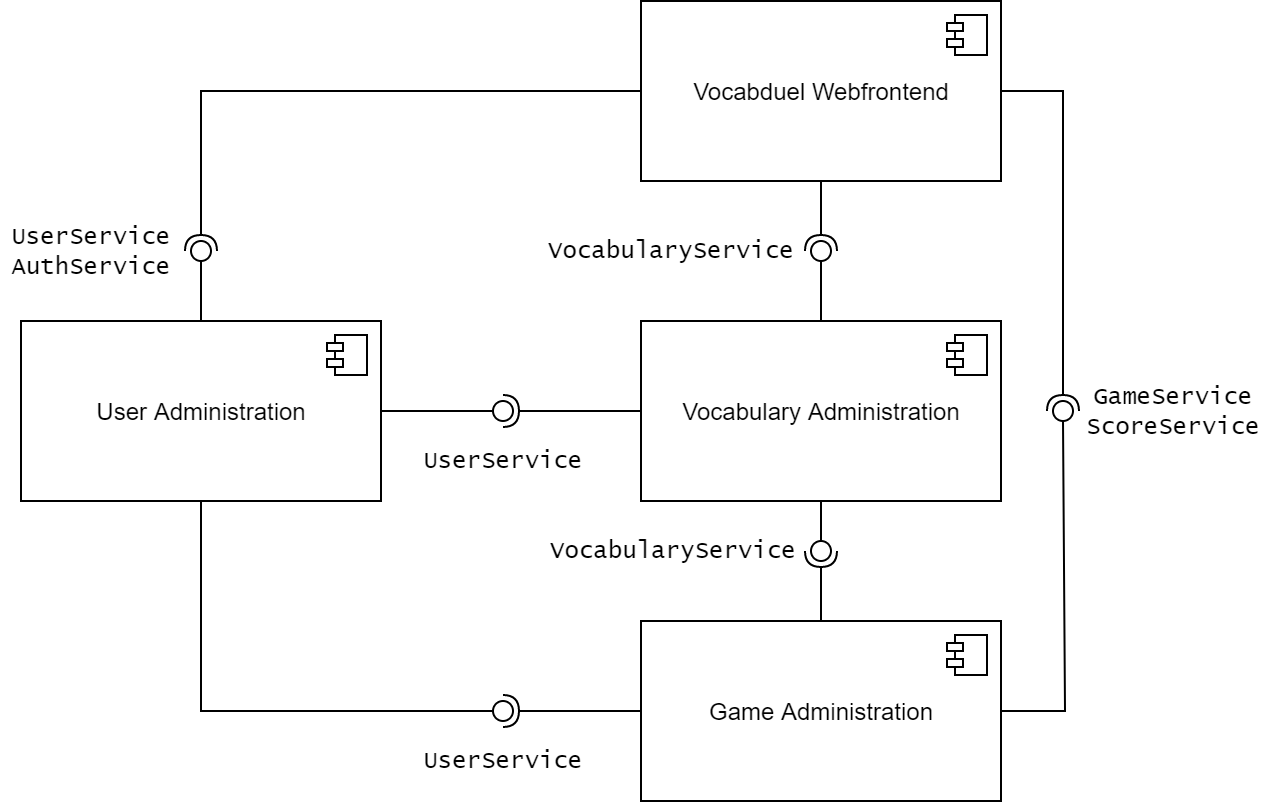
\includegraphics[width=0.8\textwidth]{components_diagram}
    \caption[]{Komponentenschnitt}
    \label{fig:komponenten-1}
\end{figure}

\subsection{Services}

Das Informationssystem lässt sich in die folgenden Services gruppieren:

\begin{outline}
    \1 \texttt{vocabulary\_administration}
    \1 \texttt{game\_administration}
    \1 \texttt{user\_administration}
\end{outline}

Das Modul \texttt{user\_administration} ist für das Nutzer-Management zuständig:
Es stellt wiederum zwei Services bereit: den \texttt{AuthService} für die Verwaltung von Zugangsdaten,
d.h.\ Passwörtern und JWT-Token, sowie den \texttt{UserService} zum Abfragen, Bearbeiten und Löschen
bestehender Nutzerdaten.

\texttt{vocabulary\_administration} ist für das Vokabel-Management zuständig:
Mithlife des \texttt{VocabularyService} wird der Zugriff sowie die Verwaltung von Vokabellisten bereitgestellt.

\texttt{game\_administration} ist für das Spiel-Management zuständig:
Durch die Bereitstellung des \texttt{GameService} wird eine Spielverwaltung zur Verfügung gestellt,
während der \texttt{ScoreService} für die Verwaltung von abgeschlossenen Spielen zuständig ist.

Alle dieser genannten Module existieren wiederum in drei Ausführungen:
\begin{outline}
    \1 Als Export-Schnittstellen, die von anderen Modulen genutzt werden können
    \1 Als tatsächliche Implementierungen, in denen die eigentliche Anwendungslogik implementiert ist und Datenbankzugriffe über DAOs erfolgen
    \1 Als Rest-Adapter, die zu ihrem jeweiligen Verantwortungsbereich eine REST-API bereitstellen
\end{outline}

\subsection{Konfigurationen und geteilte Module}\label{subsec:konfigurationen-und-geteilte-module}

Des Weiteren existieren folgende Module:

\begin{outline}
    \1 \texttt{configuration}/\texttt{configuration\_core}
    \1 \texttt{shared\_logic.rest}
    \1 \texttt{vocabduel\_ui}
\end{outline}

Zusätzlich existieren zwei Konfigurationskomponenten, wobei \texttt{configuration.rest} Spring RestEasy mit dem Angular Frontend beinhaltet und
\texttt{configuration} eine Starter-Datei (s.u.) zum Konsolen UI bereitstellt.
Beide Komponenten nutzen den über \texttt{configuration\_core} bereitgestellten Transaktionsmanager (Hibernate).
Auf diesem Weg ist eine strikte Trennung zwischen den beiden Konfigurationen möglich ohne aber mehrfache Transaktionsmanager definieren zu müssen.

Die Komponente \texttt{vocabduel\_ui} stellt das User Interface für die Configuration bereit, welches auf der Konsole ausgeführt wird.
Die Komponente \texttt{shared\_logic.rest} wird in der Rest-Schicht der Administrations-Komponenten genutzt, um RefreshToken
zur Web-Session und fehlende Daten beim API-Aufruf zu managen.



    \section{Schnittstellenbeschreibung}\label{sec:schnittstellenbeschreibung}

    \section{Konzeptionelles Datenmodell}\label{sec:konzeptionelles-datenmodell}

Das folgende Klassendiagramm ist als \texttt{svg}-Datei im Rootverzeichnis des Repositorys gespeichert (\texttt{./class-diagram.svg}).
Ebenso befindet sich dort ein zweites Klassendiagramm, das ebenfalls zusätzlich Interfaces, Exception- und Service-Klassen beinhaltet.

\begin{figure}[H]
    \centering
    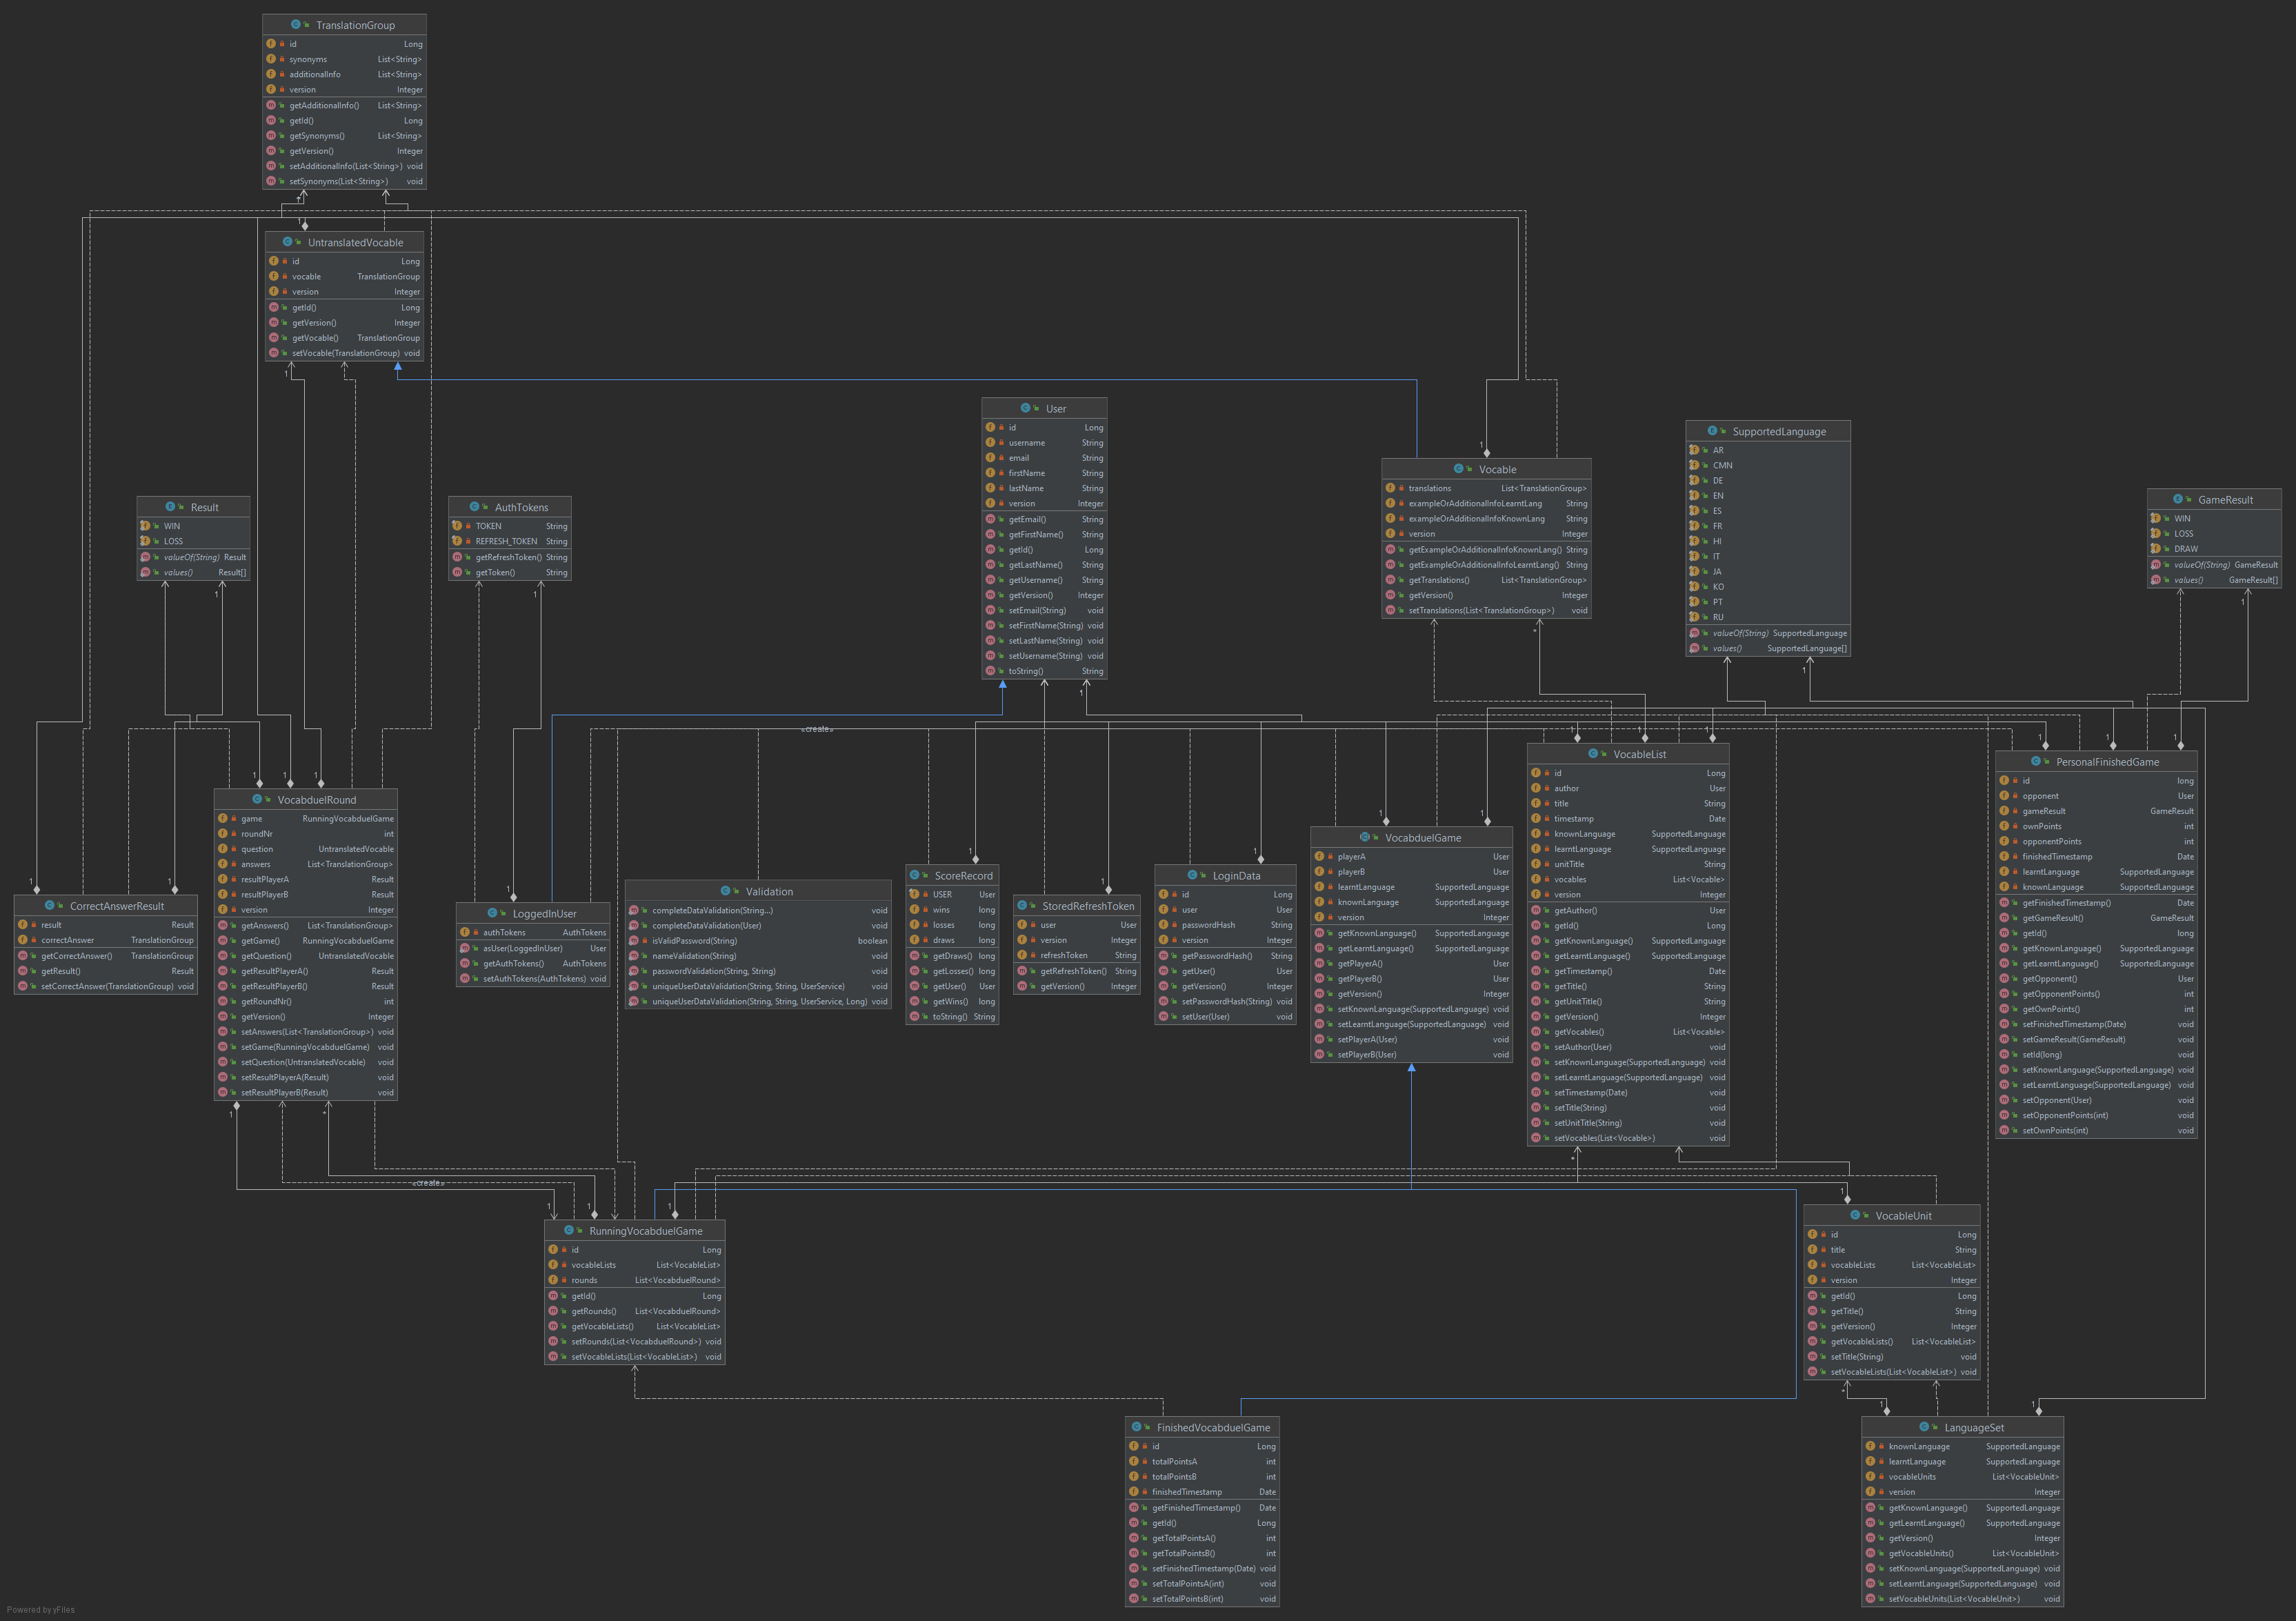
\includegraphics[width=1\textwidth]{class-diagram}
    \caption[]{Klassendiagramm}
    \label{fig:classes}
\end{figure}

Im Folgenden wird das konzeptionelle Datenmodell beschrieben, welches auch tatsächlich in ein physikalisches Datenmodell überführt wurde.

Die Entität LoginData erbt vom User Username, Email, Vor- und Zuname und speichert validierte, verschlüsselte Passwörter, die der User zum Login benötigt.
Ist der User eingeloggt, stellen die StoredRefreshToken sicher, dass der User mit gültigen Token versorgt wird, was etwa
einer gültigen Web-Session des Users auf einer Web-Applikation gleich kommt.
User mit StoredRefreshToken werden im LoggedInUser festgehalten, was aber kein Bestandteil des physikalischen Datenmodells ist.

Zur Verwaltung von Vokabellisten werden Begriffe in Synonyme und zusätzliche Informationen (additionalInfo) getrennt und in TranslationGroups einander zugeordnet.
Mit dem Erhalt einer zusätzlichen Id wird aus dem Begriff eine UntranslatedVocable.
Eine Vokabel ist schließlich die Zuordnung einer UntranslatedVocable mit anderen Begriffen.
Da UntranslatedVocable und Vocable eine gemeinsame Datenbank Tabelle darstellen,
wird zusätzlich die Spalte Datentyp (DTYPE) gestellt, um zwischen beiden Entitäten zu unterscheiden.
Beispielsatzbausteine in Lern- (UntranslatedVocable) oder Wissenssprache (Vocable) können auch in dieser Tabelle gespeichert werden.
Aus mehreren Vokabeln, Autor-Angabe, Titel und createdTimestamp wird eine Vokabelliste und aus mehreren Vokabellisten und Titel
wird eine VokabelUnit.

VokabelUnits werden mit Lern- und Wissenssprache zu einem LanguageSet.
Um mit Vokabellisten spielen zu können, werden die Spiele in RunningVocabduelGames mit Lern- und Wissenssprache sowie zwei User- und einer Vokabellist-Zuordnungen gespeichert.
Beim Spiel ist so festgehalten, welche Vokabelliste für dieses Spiel genutzt wird. Die Duell-Runden werden einzelnen Translationgroups zugeordnet, um einen Begriff zum Übersetzen zu haben.
Die möglichen Antwortmöglichkeiten zur Runde werden nicht in der Datenbank gespeichert, ebensowenig, wie die richtige Übersetzung für die Runde lautet.
Da wir die richtige Übersetzung bereits aus der Vokabel erhalten, wird für die fertig gespielte Runde nur das Ergebnis "WIN" oder "LOSS" gespeichert.
Noch laufende Runden und fertig gespielte Runden werden in derselben physikalischen Tabelle gespeichert und sind am Eintrag des Rundenergebnisses zu erkennen.
Wurden alle Runden eines Spiels gespielt, so wird ein fertig gespieltes Spiel gespeichert. Hier wird die erreichte Endpunktzahl zum Spiel von jedem Teilnehmer hinterlegt.
Ob ein Spieler damit gewonnen, verloren oder unentschieden gespielt hat, wird nicht in der Datenbank gespeichert, sondern auf dem Server ermittelt.

    \section{Präsentationsschicht}\label{sec:praesentationsschicht}

\subsection{Konsolenoberfläche}

Das Modul \texttt{configuration.rest} stellt eine einfache Konsolenoberfläche bereit.
Diese gilt allerdings als veraltet und wird daher im Folgenden nicht näher behandelt.

\subsection{Weboberfläche}

Für die Nutzung von \textit{Vocabduel} existiert eine voll funktionsfähige Webanwendung.
Diese wurde mit \textit{Angular 12} implementiert und folgt modernen Standards.

\subsubsection{Aufbau der Anwendung}

Im Folgenden werden die grundlegenden Features des \textit{Vocabduel}-Frontends erläutert.
Dabei ist jedoch zu erwähnen, dass die Anwendung nicht im Detail beschrieben wird, sondern
an dieser Stelle vielmehr ihr Aufbau und ihr Funktionsumfang skizziert werden.

\begin{figure}[H]
    \centering
    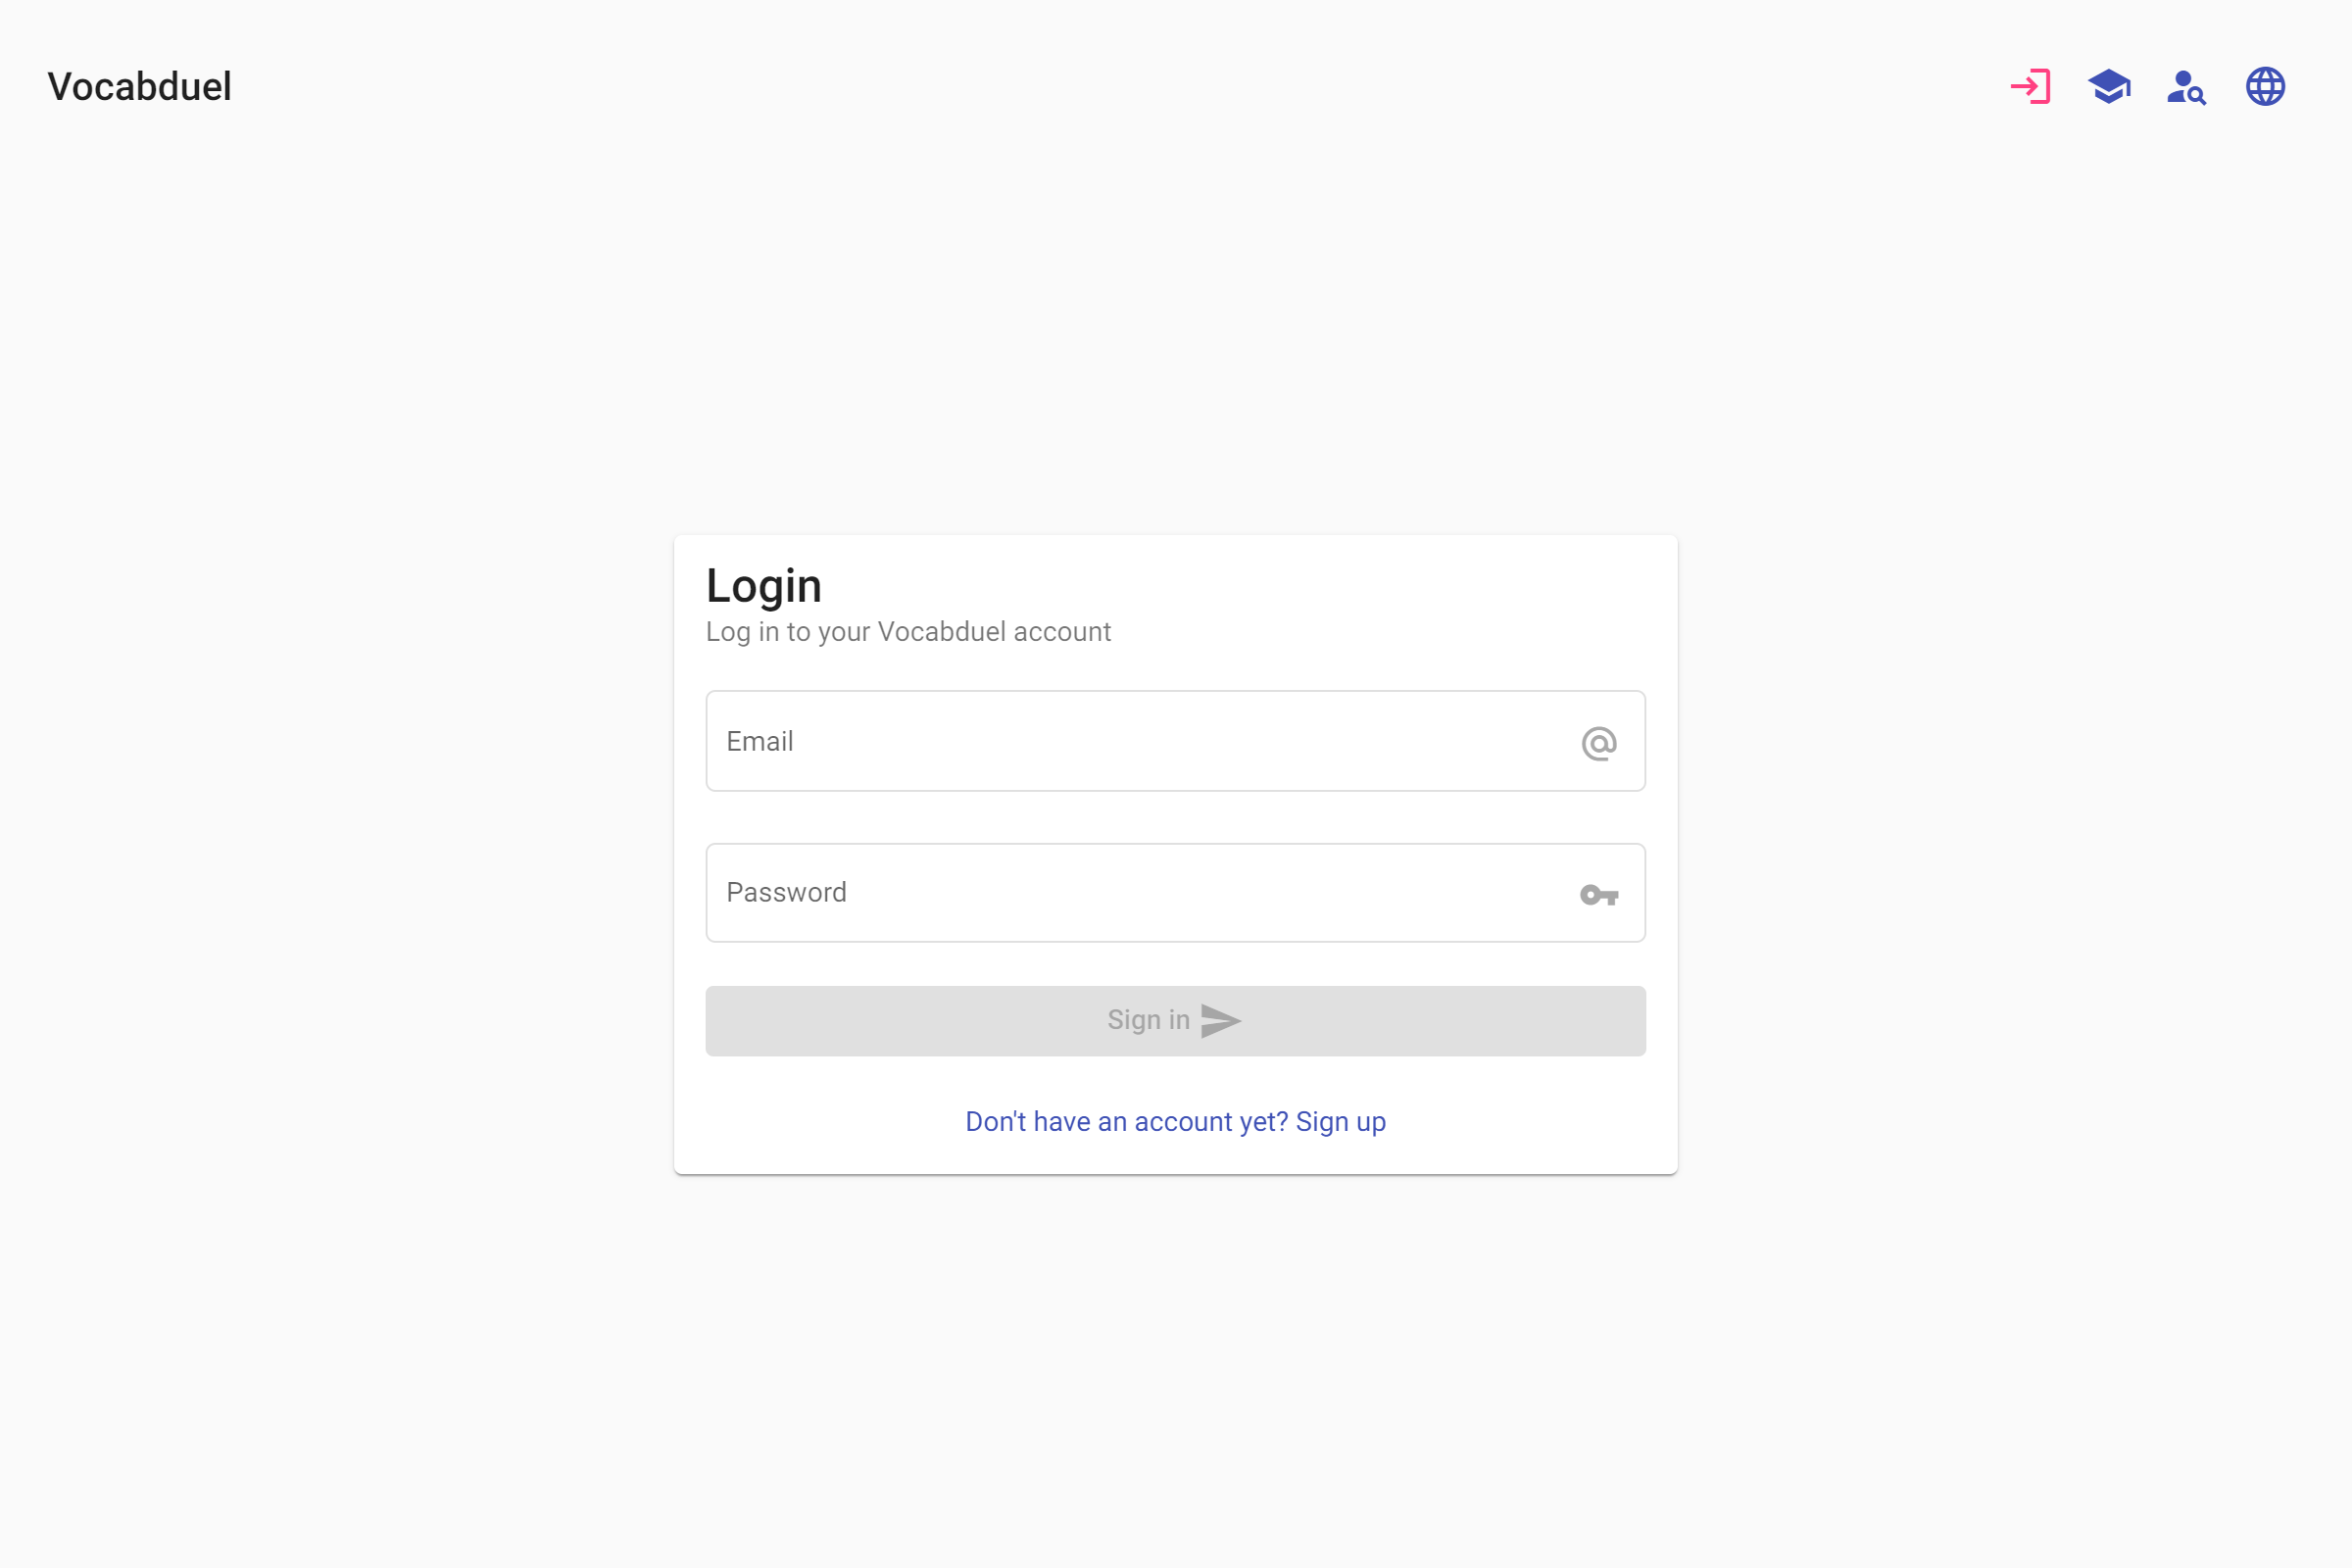
\includegraphics[width=0.8\textwidth]{localhost_8080_app_login}
    \caption[]{Login}
    \label{fig:felogin}
\end{figure}

Die Webanwendung verfügt über eine Oberfläche mithilfe derer man sich im System anmelden kann.
Analog zum Login existiert auch eine Seite zum Erstellen eines Kontos.
Über die Icons in der rechten, oberen Ecke kann zu weiteren Seiten navigiert werden.

\begin{figure}[H]
    \centering
    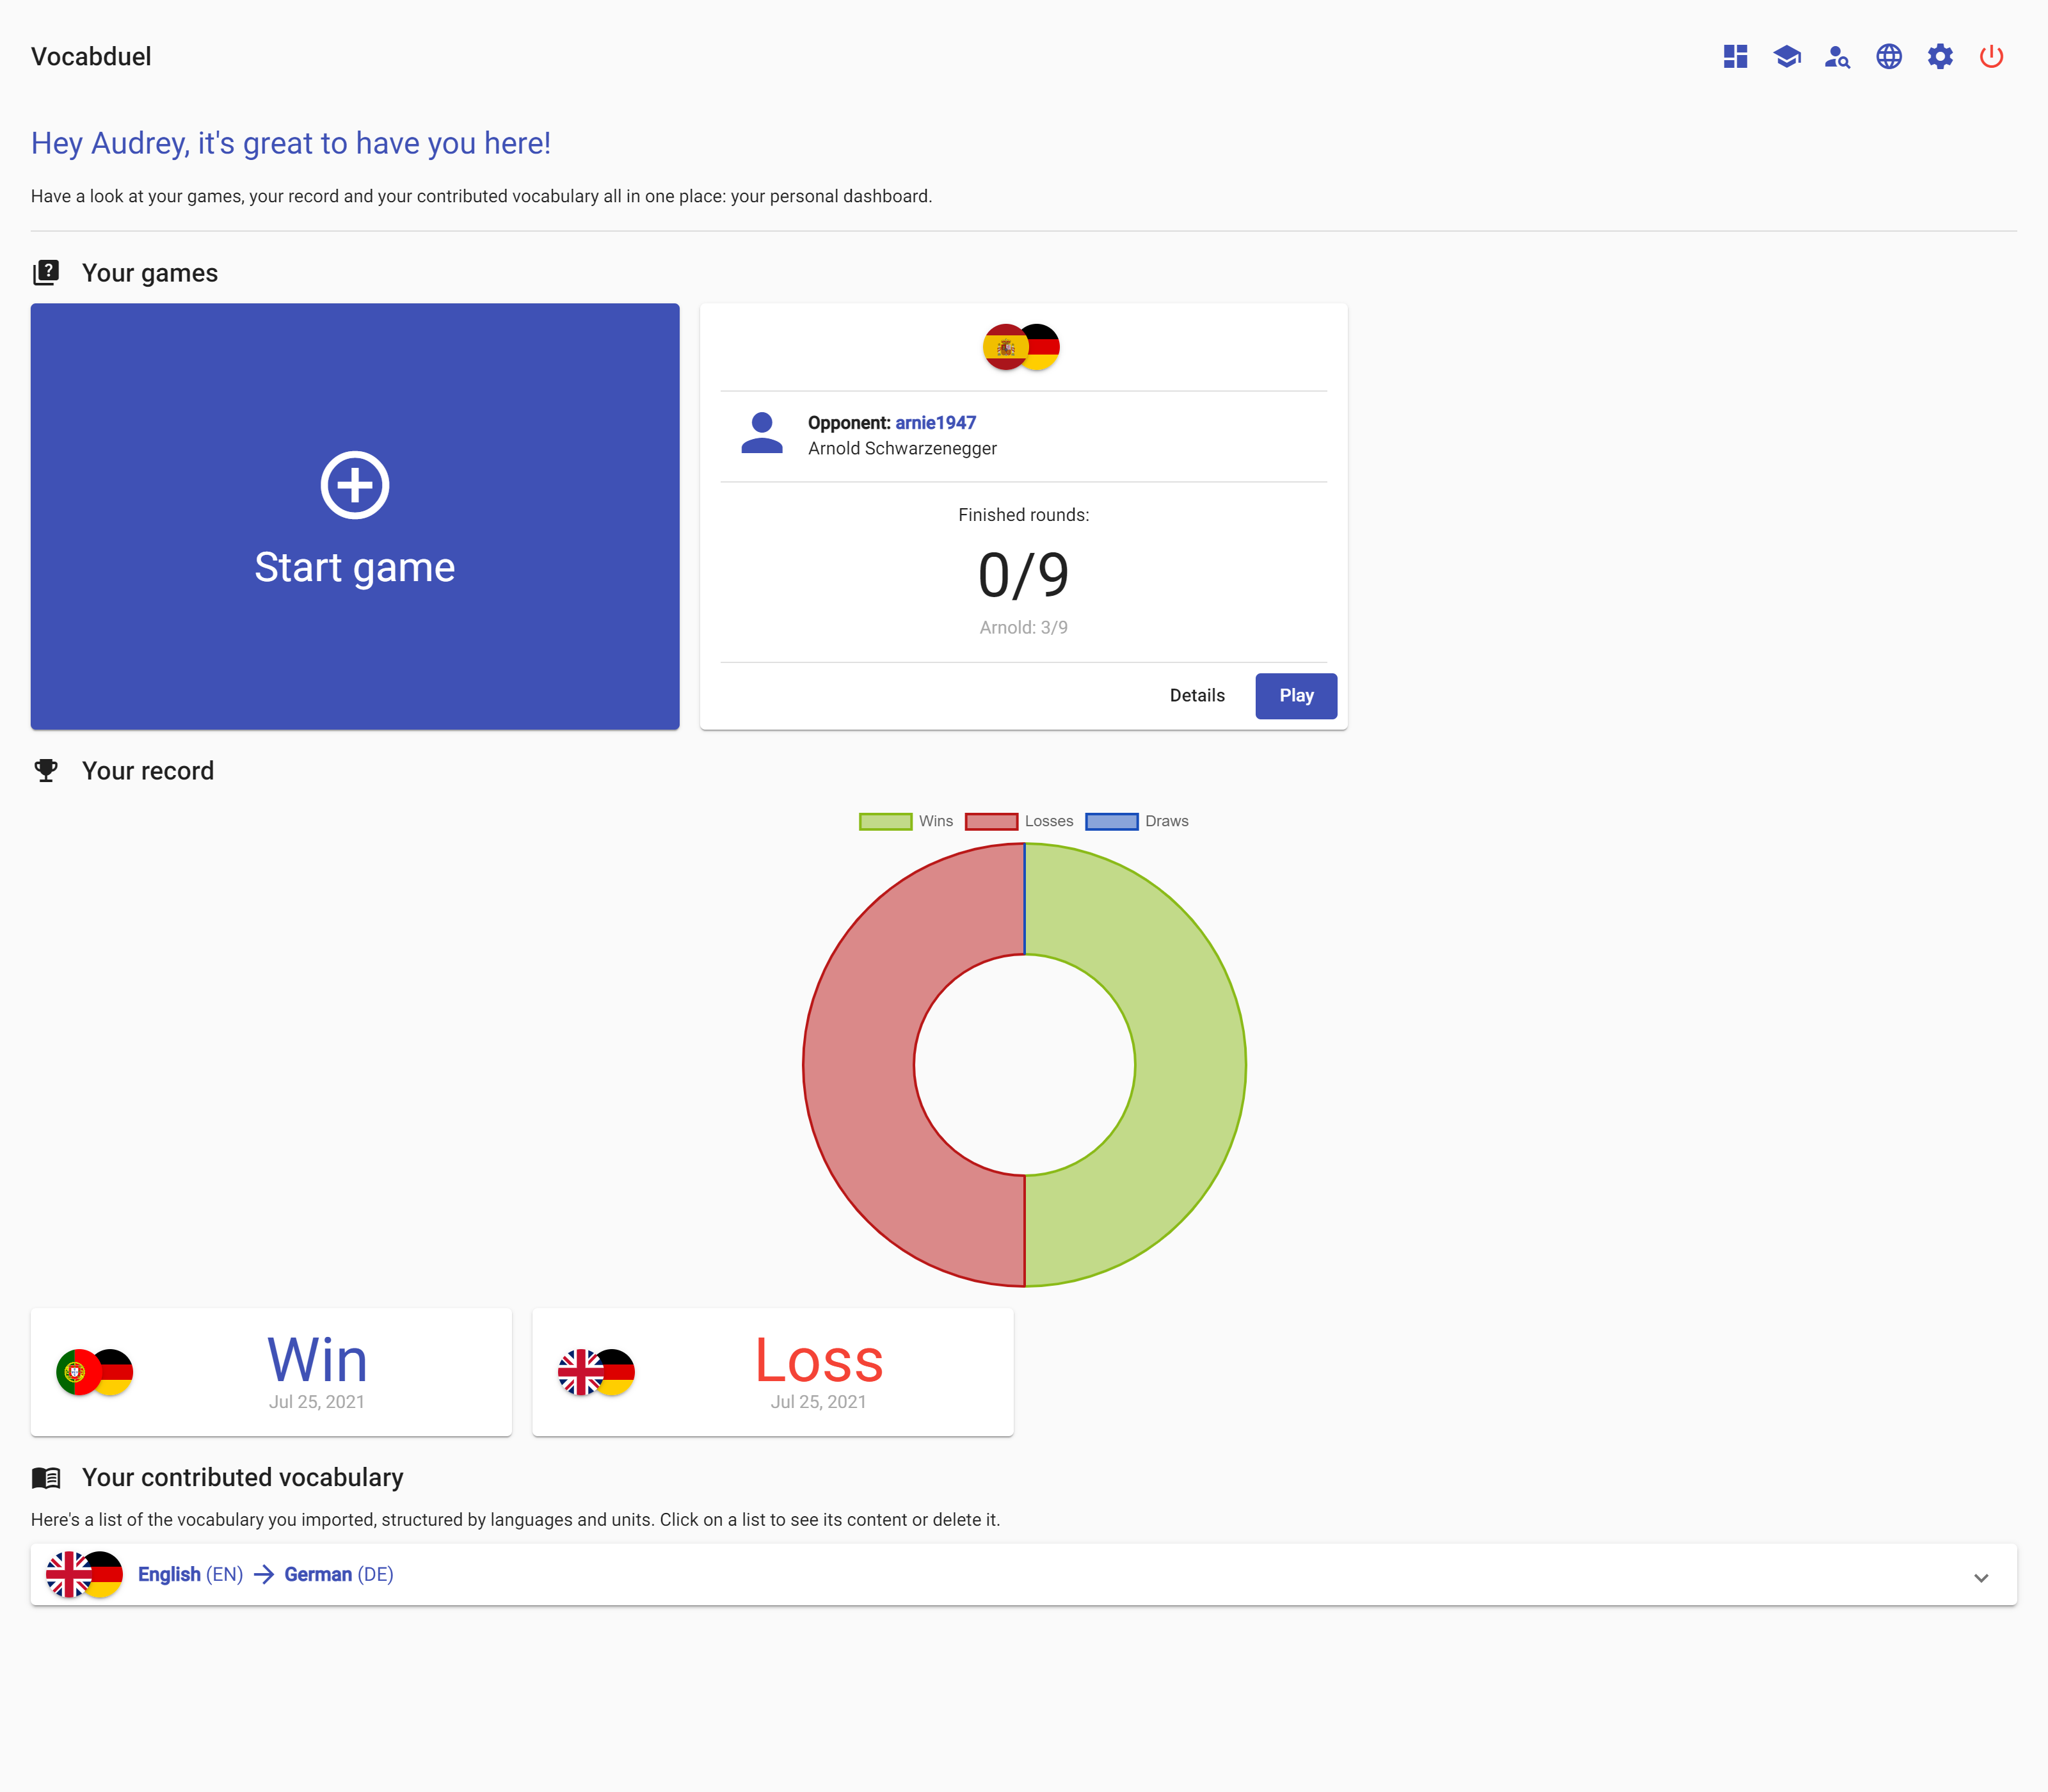
\includegraphics[width=0.8\textwidth]{localhost_8080_appdashboard (1)}
    \caption[]{Dashboard}
    \label{fig:fedashboard}
\end{figure}

Sobald eingeloggt, besteht Zugriff auf das persönliche Dashboard, das aktuelle Spiele, Spielergebnisse sowie eine Übersicht
über vom angemeldeten Nutzer importierte Vokabellisten beinhaltet.

\begin{figure}[H]
    \centering
    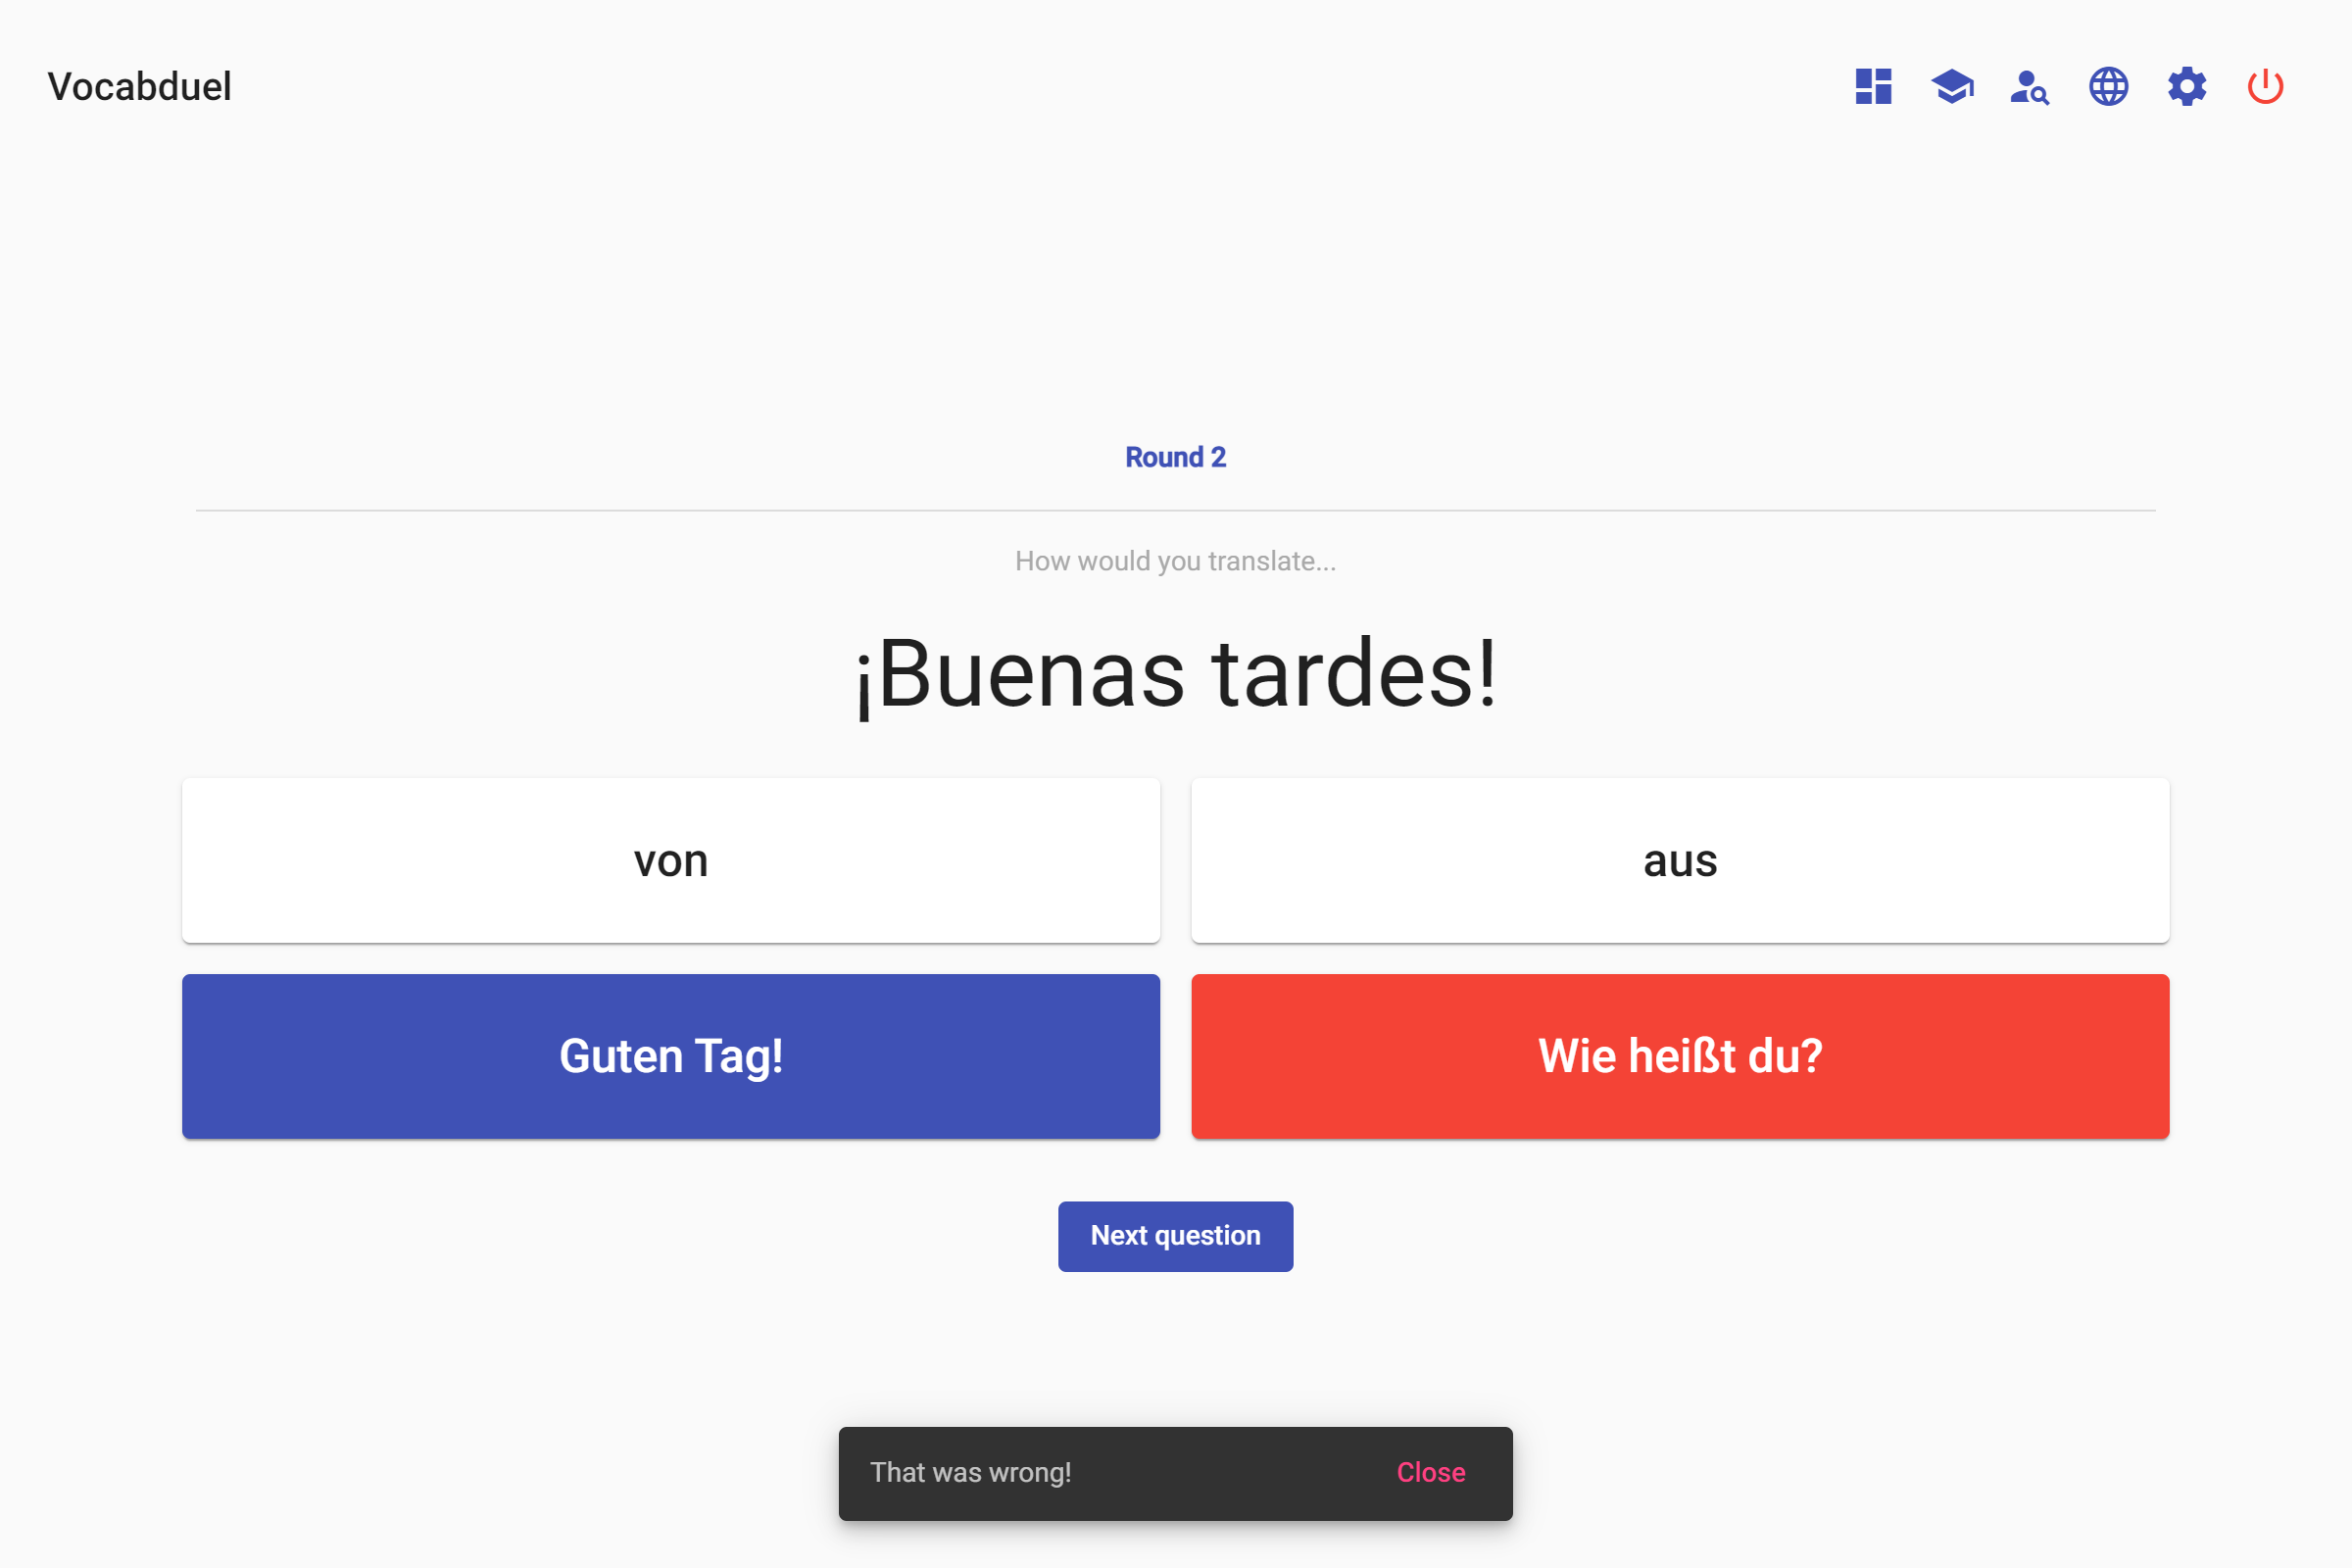
\includegraphics[width=0.8\textwidth]{localhost_8080_app_login (2)}
    \caption[]{Beantworten einer Frage}
    \label{fig:fegame}
\end{figure}

Vom Dashboard aus kann entweder ein existierendes Spiel geöffnet oder ein neues Spiel gestartet werden.
Nach dem Einreichen einer Antwort erfolgt direktes Feedback und die nächste Runde (sofern vorhanden) kann
gespielt werden.

\begin{figure}[H]
    \centering
    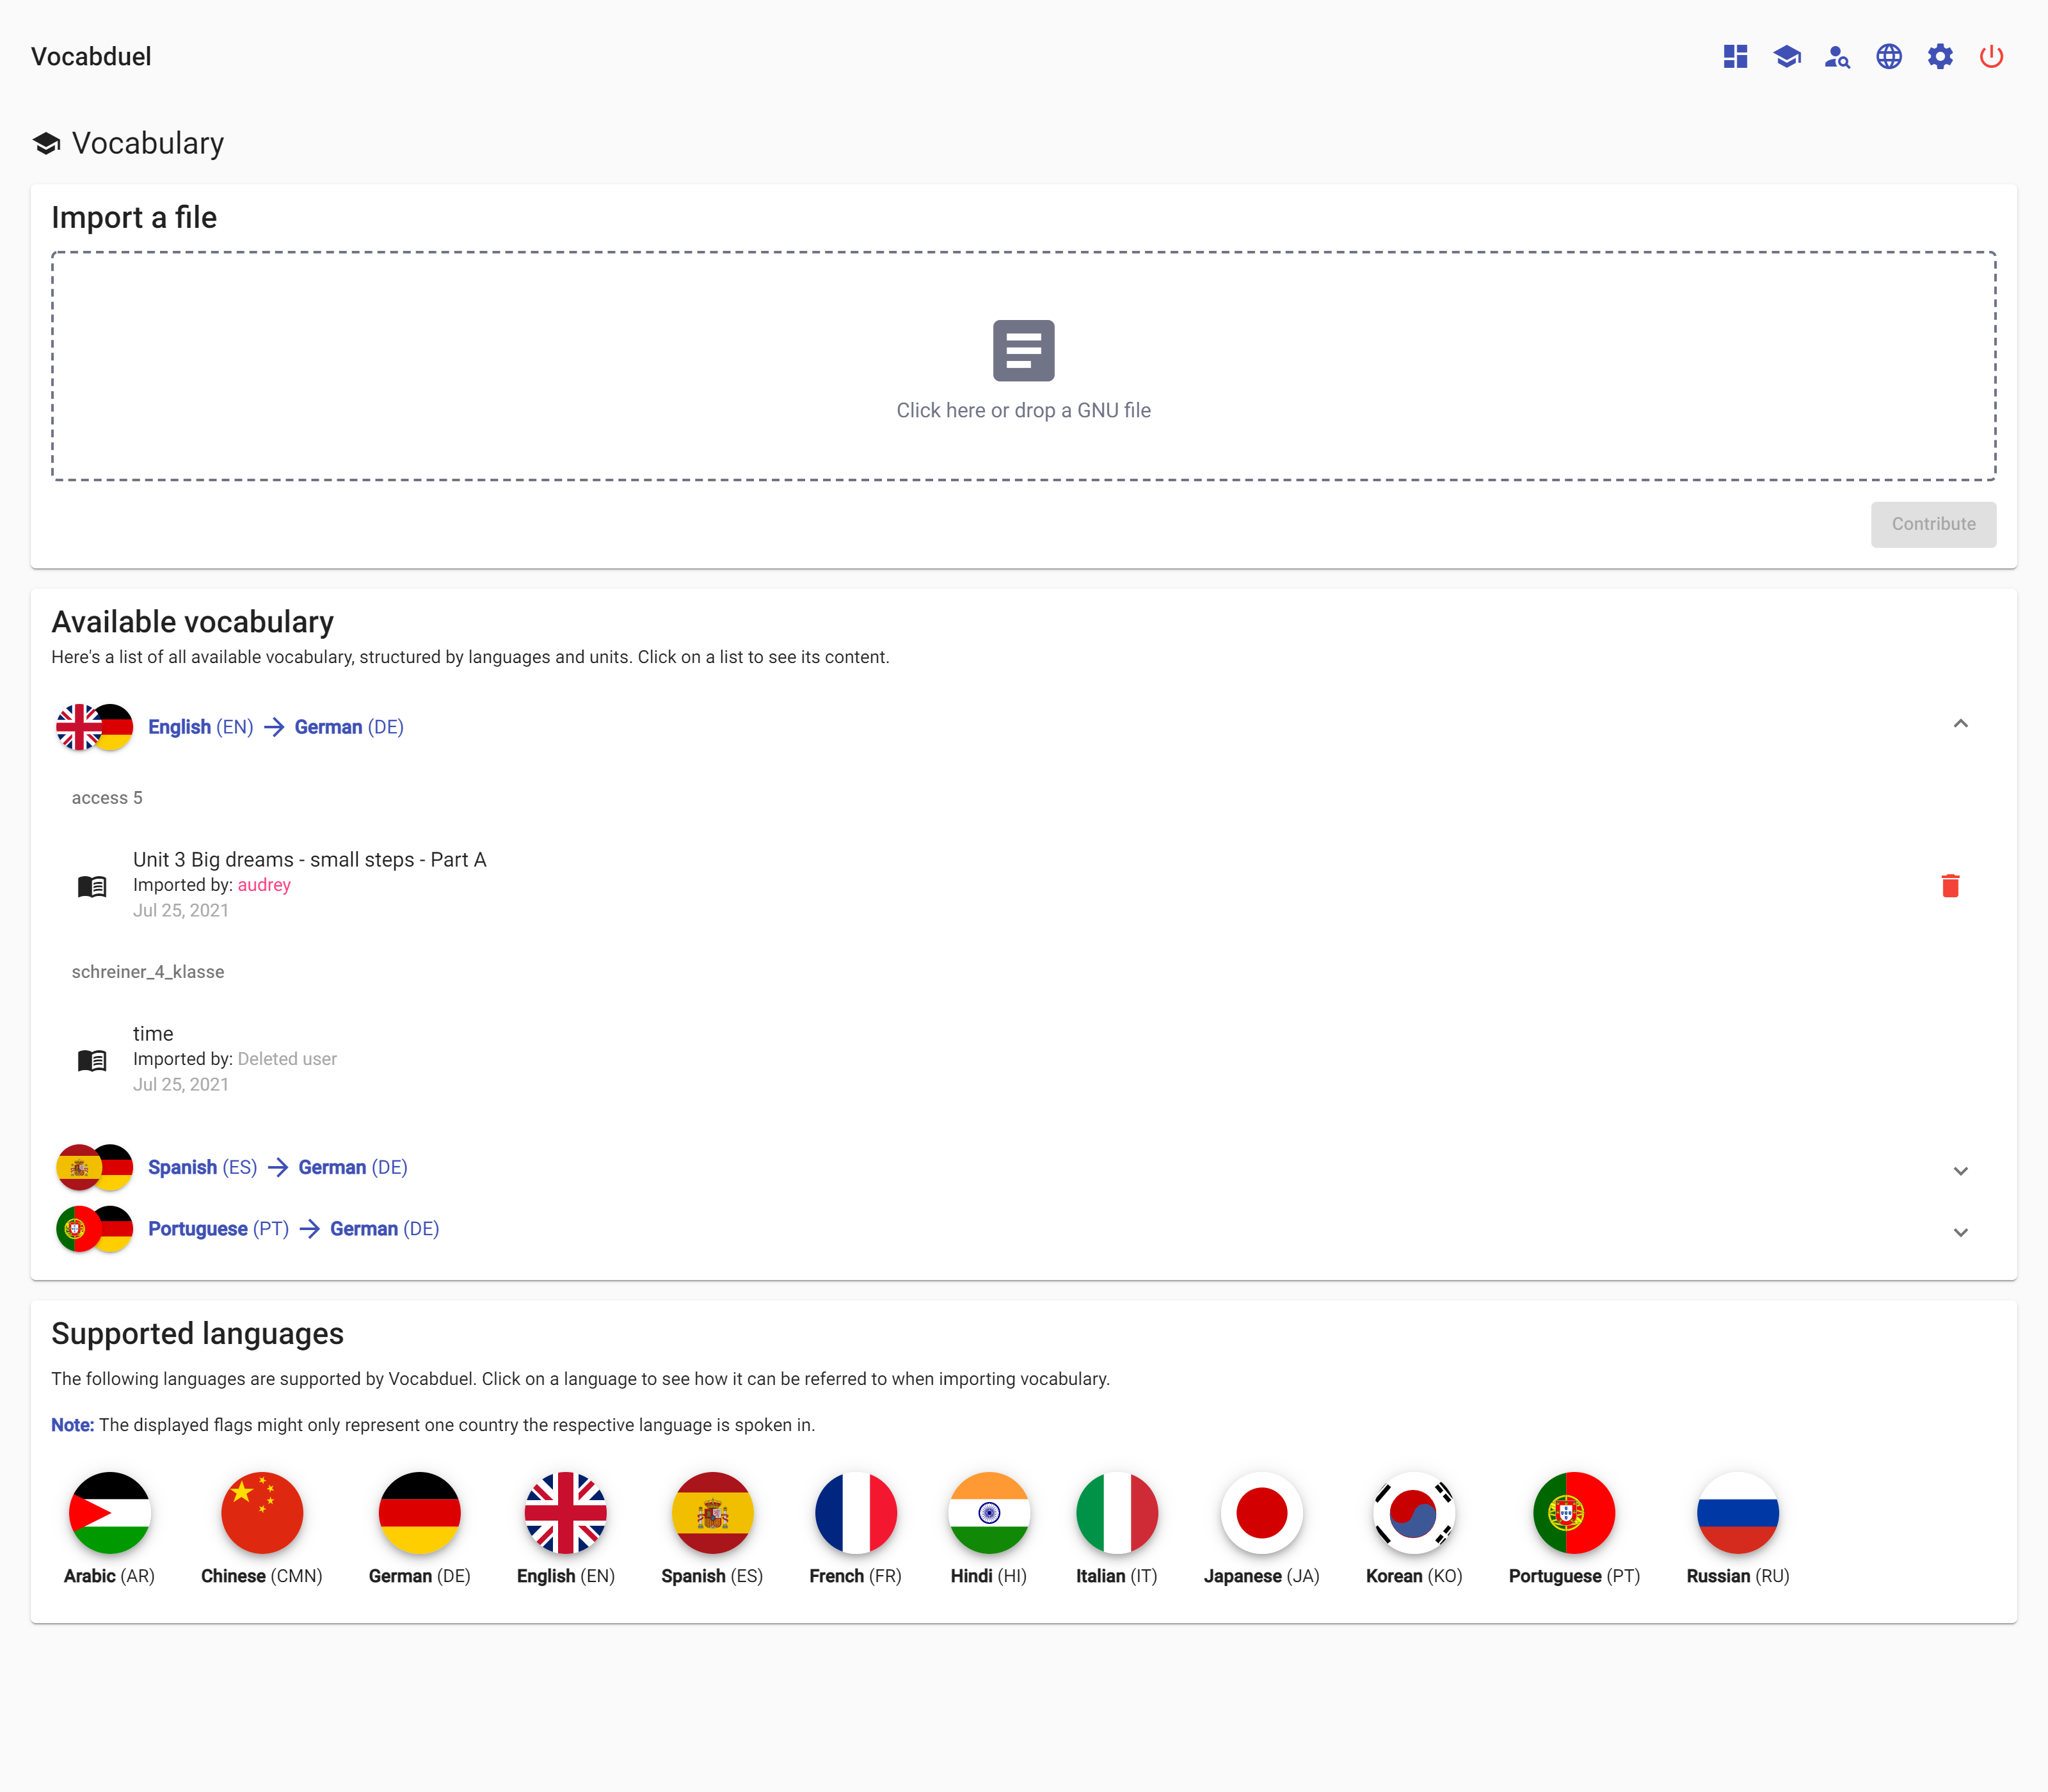
\includegraphics[width=0.8\textwidth]{localhost_8080_app_vocab}
    \caption[]{Vokabelmanagement}
    \label{fig:fevocab}
\end{figure}

Die Vokabelmanagement-Seite zeigt alle importierten Vokabellisten, gruppiert nach Sprachen und Units sowie alle vom System
unterstützen Sprachen für Vokabellisten.
Grundsätzlich ist sie ohne vorherige Authentifizierung zugänglich, in diesem Fall könnten allerdings keine neuen Vokabellisten importiert werden (vgl.\ Abbildung~\ref{fig:fevocab}).

\begin{figure}[H]
    \centering
    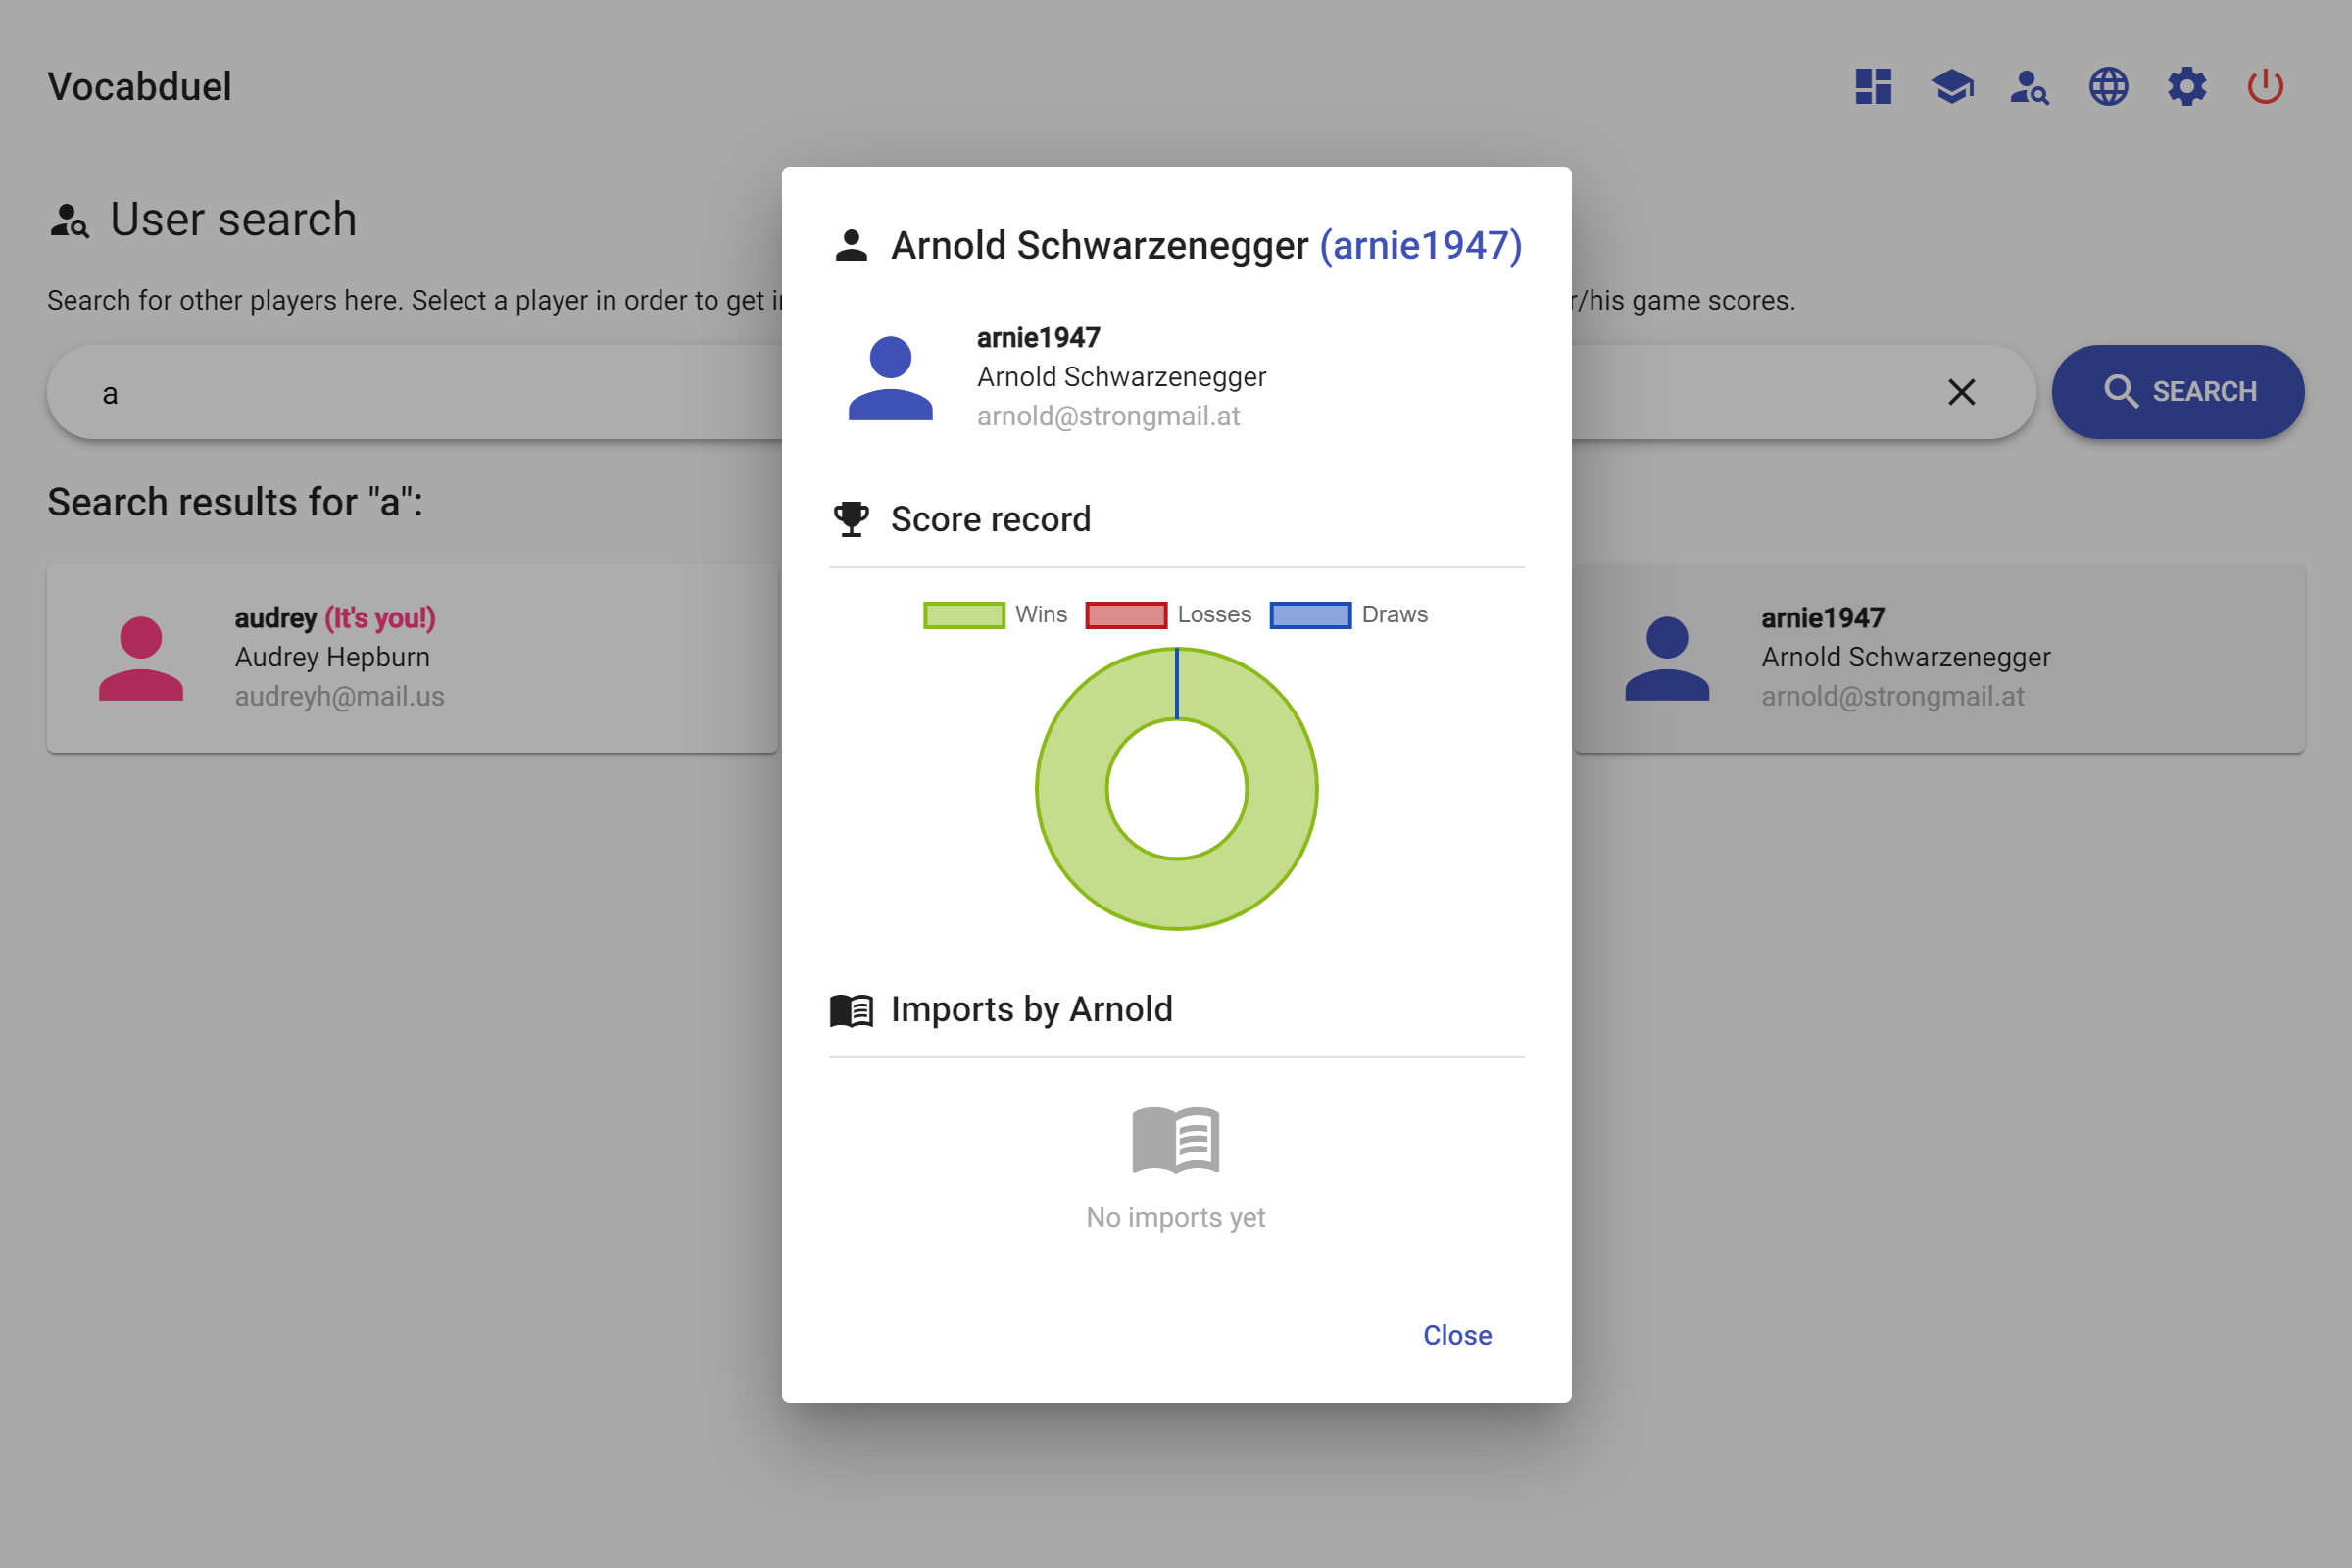
\includegraphics[width=0.8\textwidth]{localhost_8080_app_search}
    \caption[]{Details zu einer gesuchten Person}
    \label{fig:fesearch}
\end{figure}

Ähnlich ist die Suche nach Nutzern frei zugänglich.
Die Spielergebnisse einer Person sehen zu dürfen, setzt allerdings eine Authentifizierung voraus, während von der ausgewählten Person importierte Listen öffentlich einsehbar sind.
Um Details zu einem Datensatz wie einem Spiel, einer Vokabelliste oder, wie hier, einer Person einzusehen, finden in der Anwendung Dialoge Verwendung.

\begin{figure}[H]
    \centering
    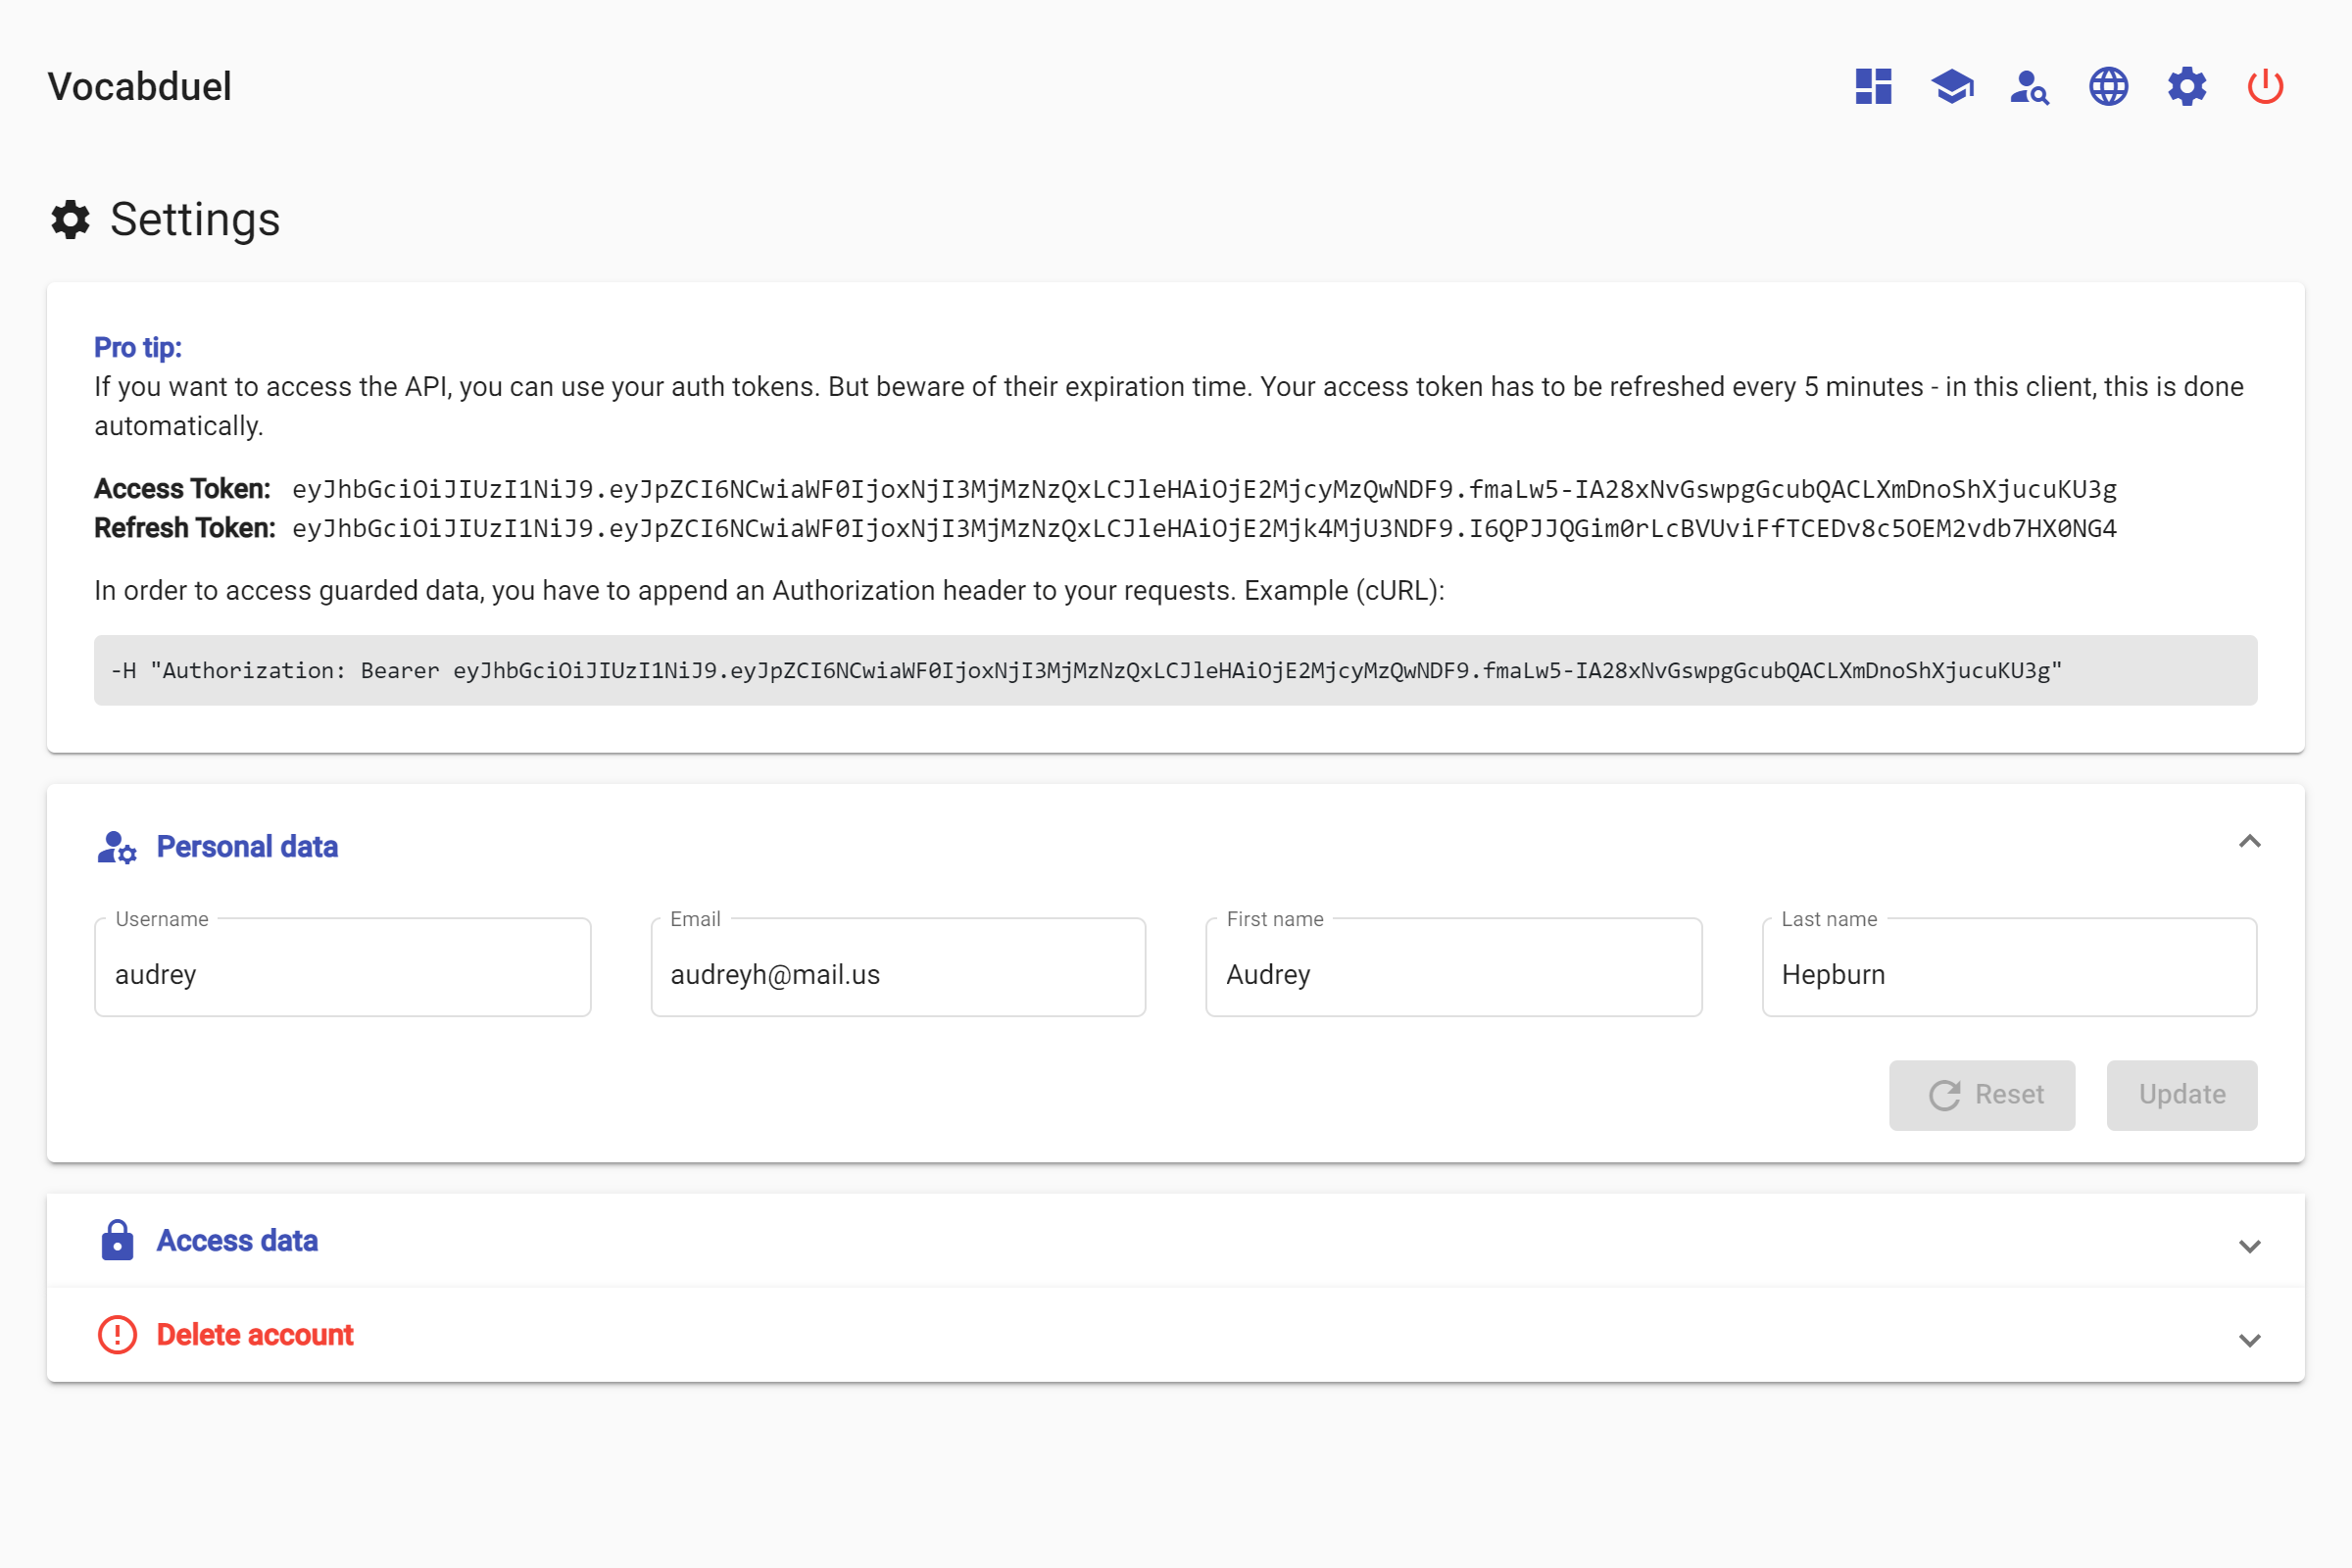
\includegraphics[width=0.8\textwidth]{localhost_8080_app_login (1)}
    \caption[]{Nutzereinstellungen}
    \label{fig:fesettings}
\end{figure}

Sofern authentifiziert, besteht zudem die Möglichkeit, persönliche Daten über die Nutzereinstellungen zu konfigurieren.

\subsubsection{Struktur aus Entwicklungssicht}

Aus Entwicklungssicht besteht die Anwendung aus:

\begin{itemize}
    \item \textbf{Components:} Anzuzeigende Komponenten, die jeweils aus einer \textit{HTML}-, einer \textit{SCSS-}
    und einer \textit{TypeScript}-Datei bestehen. Diese sind beliebig wiederverwertbar und lassen sich ineinander verschachteln.
    Zusammengefasst sind somit alle dargestellten Bestandteile der Anwendung Components, die Teil der \texttt{AppComponent} sind.
    \item \textbf{Directives:} Klassen, die dargestellte Elemente um Logik erweitern. In der konkreten Anwendung gibt es lediglich
    eine Directive, die zu langen Text automatisch abbricht und durch "..." ersetzt.
    \item \textbf{Guards:} Interfaces, die prüfen, ob eine bestimmte Route aktiviert werden kann und sollte die hierfür
    aufgestellte Bedingung nicht erfüllt sein, auf eine andere Seite weiterleiten. Ein Beispiel wäre die Login-Seite, die nur
    dann aufgerufen werden kann, wenn keine Person in der aktuellen Session eingeloggt ist. Auch lassen sich für eine Route mehrere
    Guards definieren.
    \item \textbf{Helpers:} Nicht direkt zuordenbare Hilfsklassen. In der konkreten Anwendung gibt es nur eine derartige
    Klasse, die die Authentifizierungslogik für jegliche Requests übernimmt.
    \item \textbf{Model:} Klassen, die die Struktur der verarbeiteten bzw. dargestellen Informationen definieren.
    \item \textbf{Pipes:} Klassen, die dazu dienen, anzuzeigende Werte zu transformieren.
    \item \textbf{Services:} Per DI injizierbare und somit als Singleton nutzbare Klassen, die grundlegende, gemeinsam genutzte
    Logik bereitstellen. In dieser Anwendung ist für jedes REST-Modul eine derartige Serviceklasse definiert, um alle HTTP-Requests
    zentral zu definieren und von den angezeigten Komponenten zu trennen. Weitere Logik wie eine zentrale Verwaltung zum Speichern
    von Daten oder der Sprachenverwaltung (Internationalisierung) ist auch über Serviceklassen realisiert.
\end{itemize}

Das \textit{Vocabduel}-Frontend wurde zunächst als gesondertes Projekt behandelt, im Laufe der Zeit allerdings in das Mono-Repository integriert.
Die Gründe hierfür werden in Kapitel~\ref{sec:ablaufumgebung} näher erläutert.

\subsubsection{Kommunikation mit REST-Schnittstellen}

Die folgende Liste gibt Auskunft darüber, welche REST-Adapter zu welchem Zeitpunkt von der Webanwendung angesprochen werden bzw.\ durch Nutzerinteraktionen ansprechbar sind:

\begin{outline}
    \1 \textbf{\texttt{AuthServiceRestAdapter}}
    \2 \texttt{/register} : Registrierungsseite
    \2 \texttt{/login} : Loginseite
    \2 \texttt{/current-user} : \textit{(Anzahl an Requests durch clientseitiges Caching eingeschränkt)}
    \3 Jede Seite, die Authentifizierung erfordert
    \3 Guards zum Prüfen, ob authentifiziert
    \2 \texttt{/refresh-token} : Im Hintergrund bei Error \texttt{401} (\texttt{AuthInterceptor})
    \2 \texttt{/update-password} : Nutzereinstellungen

    \1 \textbf{\texttt{UserServiceRestAdapter}}
    \2 \texttt{/find} :
    \3 Seite zur Suche nach Personen
    \3 Dialog für die Festlegung eines Gegners beim Starten eines Spiels
    \2 \texttt{/get} : Dialog für die Festlegung eines Gegners beim Starten eines Spiels
    \2 \texttt{/update-account} : Nutzereinstellungen

    \1 \textbf{\texttt{VocabularyServiceRestAdapter}}
    \2 \texttt{/list/\{id\}} : Vokabelliste-Dialog, wenn von Spieldetails aus geöffnet
    \2 \texttt{/lists-of-author/\{id\}} :
    \3 Dashboard (eigene Listen)
    \3 User-Details-Dialog
    \2 \texttt{/language-sets} :
    \3 Vokabelmanagement-Seite
    \3 Dialog zur Auswahl von Vokabellisten beim Starten eines Spiels
    \2 \texttt{/language-references/\{lang\}} : Vokabelmanagement-Seite
    \2 \texttt{/supported-languages} : Vokabelmanagement-Seite
    \2 \texttt{/import-gnu} : Vokabelmanagement-Seite
    \2 \texttt{/delete-list/\{listId\}} :
    \3 Vokabelmanagement-Seite
    \3 Dashboard (eigene Listen)

    \1 \textbf{\texttt{GameServiceRestAdapter}}
    \2 \texttt{/finish-game} : Seite mit laufendem Spiel
    \2 \texttt{/finished-games} : Dashboard
    \2 \texttt{/record} : Dashboard
    \2 \texttt{/record/{userId}} : User-Details-Dialog

    \1 \textbf{\texttt{GameServiceRestAdapter}}
    \2 \texttt{/start} : Seite zum Starten eines Spiels
    \2 \texttt{/open-games} : Dashboard
    \2 \texttt{/current-round/\{gameId\}} : Seite mit laufendem Spiel
    \2 \texttt{/answer/\{gameId\}/\{roundNr\}} : Seite mit laufendem Spiel
    \2 \texttt{/delete-account-and-game-widows} : Nutzereinstellungen

\end{outline}

\textbf{Anmerkung:} Das Löschen von Nutzerdaten über \texttt{GameServiceRestAdapter} zu steuern, ermöglicht es, direkt
alle zugehörigen offenen Spiele der gelöschten Person zu entfernen.

\subsubsection{Fehlerbehandlung}

In der Anwendung existiert ein zentraler Service, der alle unbehandelten Fehler abfängt (\texttt{ErrorService}), für die abhängig vom Statuscode (sofern vorhanden) einen
bestimmten, generischen Dialog anzeigt.

\begin{figure}[H]
    \centering
    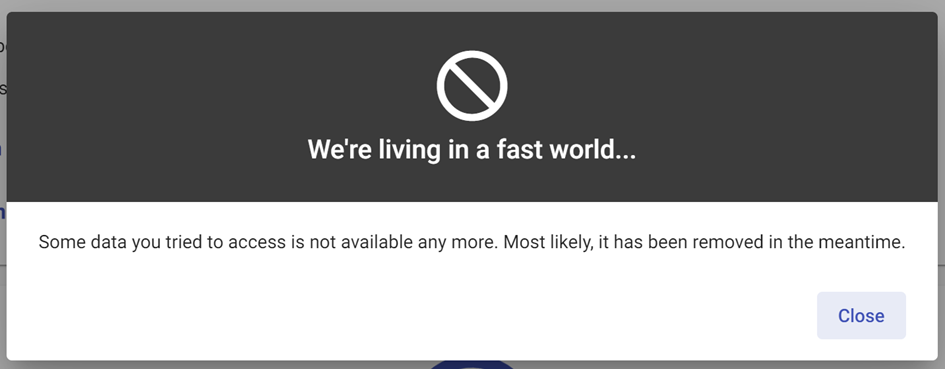
\includegraphics[width=0.8\textwidth]{404-dialog}
    \caption[]{Generische Behandlung eines \texttt{Not Found} Errors (404)}
    \label{fig:404}
\end{figure}

\begin{figure}[H]
    \centering
    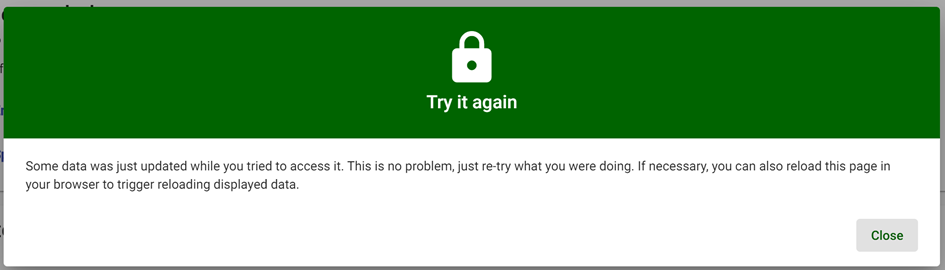
\includegraphics[width=0.8\textwidth]{412-dialog}
    \caption[]{Generische Behandlung eines \texttt{Precondition Failed} Errors (412)}
    \label{fig:412}
\end{figure}

\begin{figure}[H]
    \centering
    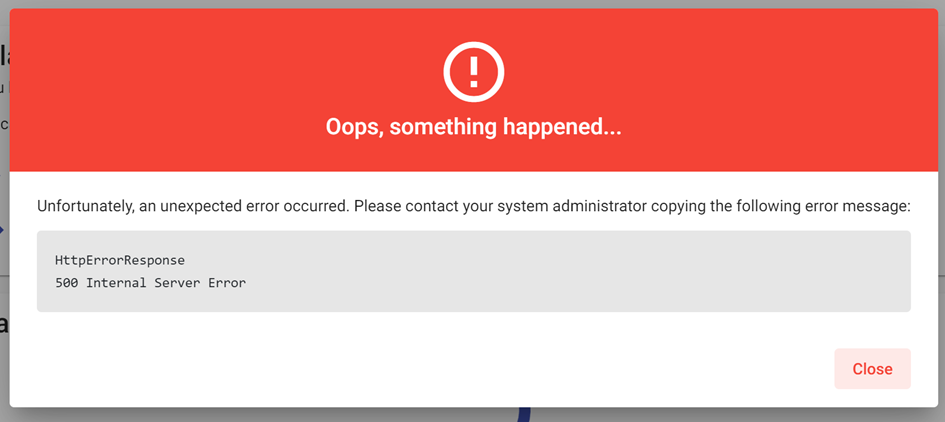
\includegraphics[width=0.8\textwidth]{500-dialog}
    \caption[]{Generische Behandlung eines unerwarteten Fehlers, in diesem Beispiel \texttt{Internal Server Error (500)} (anzunehmender Regelfall)}
    \label{fig:500}
\end{figure}

Darüber hinaus werden \texttt{Bad Request} Errors (400) in der Regel wie folgt behandelt:

\begin{figure}[H]
    \centering
    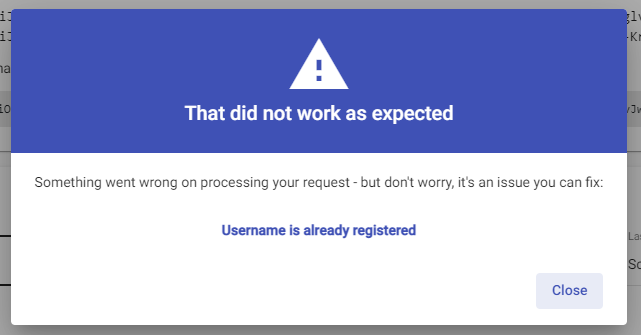
\includegraphics[width=0.8\textwidth]{400-dialog}
    \caption[]{Typische Behandlung eines \texttt{Bad Request} Errors (400)}
    \label{fig:400}
\end{figure}

\subsubsection{Weitere Features}

Die Anwendung ist so implementiert, dass sie sowohl auf kleinen als auch auf großen Bildschirmen verwendet werden kann (Responsive Design)
und orientiert sich in ihrer allgemeinen Erscheinung stark an Guidelines und Best Practices zu Material Design.

Des Weiteren ist die Applikation aktuell nur auf Englisch verfügbar, allerdings durch das Auslagern von Strings sowie einen vollständig implementierten
Service zum Verwalten von Sprachdateien (\texttt{I18nService}) leicht in andere Sprachen zu übersetzen.

\subsection{Postman Collection}

Zum Testen der API ist auch eine \textit{Postman}-Collection mit vordefinierten Requests im Rootverzeichnis des Repositorys hinterlegt.
Für Nutzer mit den IDs 2, 4 und 6, die in den ersten Requests angelegt werden, sind Tokens mit einer Gültigkeit von
5 Jahren konfiguriert, um die eigentlich implementierte regelmäßige Neuauthentifizierung bei der Nutzung der Collection zu umgehen.

    \section{Frameworks}\label{sec:frameworks}

Für dieses Java Maven-Projekt wurde Hibernate genutzt, um aus den models
eine MySQL Datenbank anzulegen und zu verwalten.
Dafür wurde den models Klassen die Annotation @Entity und den Klassenattributen, welche
in der Datenbank Tabellenspalten darstellen sollen, die Annotation @Id, @Column oder @ElementCollection gegeben.
Für Tabellen-Joins wurden die Annotationen @OneToMany, @ManyToOne und @OneToOne genutzt.

\begin{figure}[H]
    \centering
    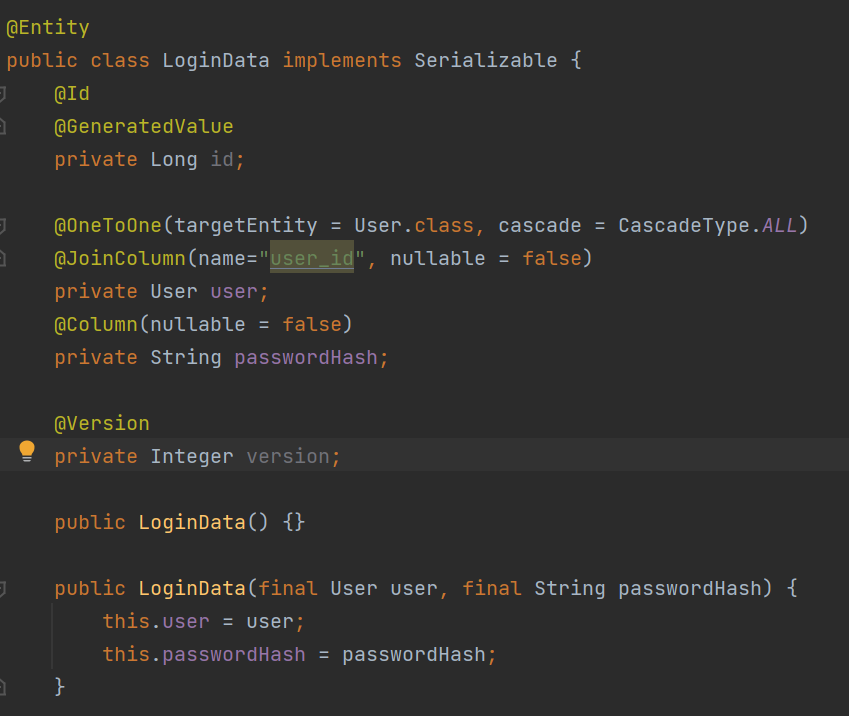
\includegraphics[width=0.8\textwidth]{user-entity}
    \caption[]{Beispiel für annotierte Model-Klasse (LoginData)}
    \label{fig:user-entity}
\end{figure}

Die EntityManagerFactory greift auf die persistence.xml zu, in der wiederum definiert ist, auf welche MySQL Datenbank mit welchem User wie zugegriffen
und welche models zur Datenbankerzeugung genutzt werden sollen.
Zudem wird der HibernateTransactionManager genutzt, dem dieses Mal über eine Bean die Information injiziert wird,
mit welchem User auf welche MySQL-Datenbank zugegriffen werden soll.
Der HibernateTransactionManager besitzt per default einen EntityManager, der
über die Annotation @PersistenceContext in die DAOs injected wird.

\begin{figure}[H]
    \centering
    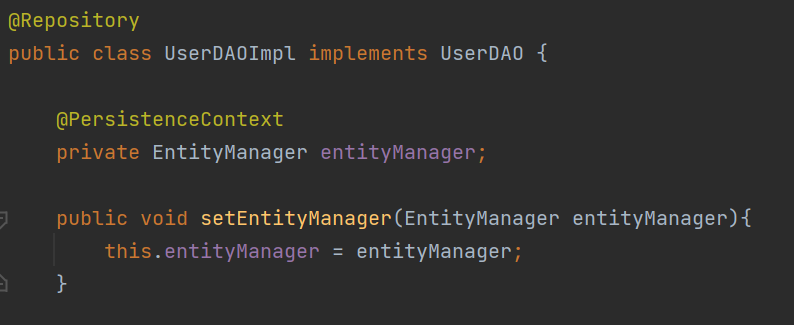
\includegraphics[width=0.8\textwidth]{user-dao-with-pc}
    \caption[]{DAO-Klasse mit Annotation \texttt{PersistenceContext} (UserDAOImpl)}
    \label{fig:userdao}
\end{figure}

Auf einem Tomcat Server der Version 9.0.40 läuft der Spring RestEasy Server, welcher
in der Rest-Schicht des configuration Moduls konfiguriert wird.
Die Rest-Schichten der Module game\_administration, user\_administration und vocabulary\_administration
wurden als Dependencies angegeben und die Beans, in denen die REST HTTP Methoden definiert sind,
dem Server hinzugefügt.

Für die Benutzeroberfläche wird Angular genutzt.
Dazu wird im Maven Executions node, npm und Angular installiert und das Angular Projekt gestartet.

\begin{figure}[H]
    \centering
    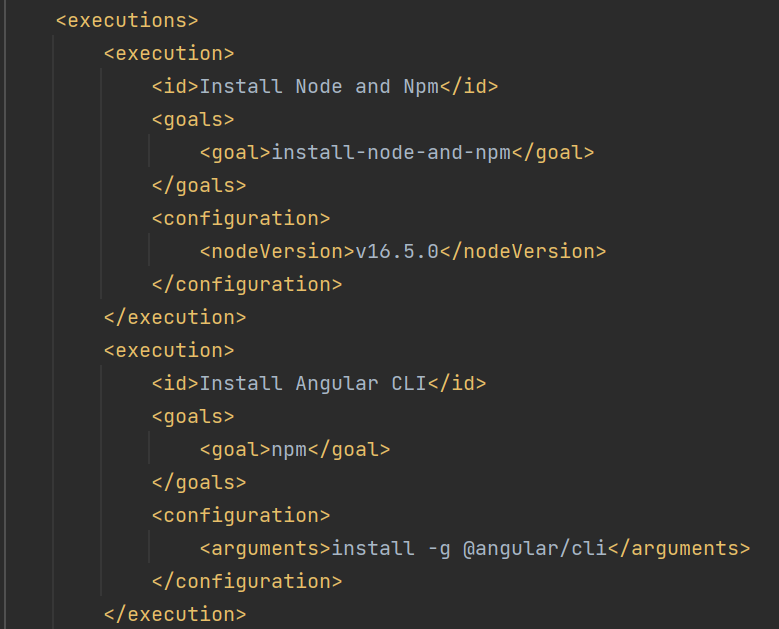
\includegraphics[width=0.8\textwidth]{snipped-plugin}
    \caption[]{Ausschnitt aus Build-Plugin zum Bauen des Frontends}
    \label{fig:snippet}
\end{figure}

Die JUnit Tests werden mit dem Mockito Framework durchgeführt.
Normalerweise wird der MockitoJUnitRunner genutzt, um die Tests zu starten.
Mithilfe der Annotation @Mock und dem Methodenaufbau Mockito.when().thenReturn(); werden
Klassen, Methodenaufrufe und Returnwerte gemockt.

\begin{figure}[H]
    \centering
    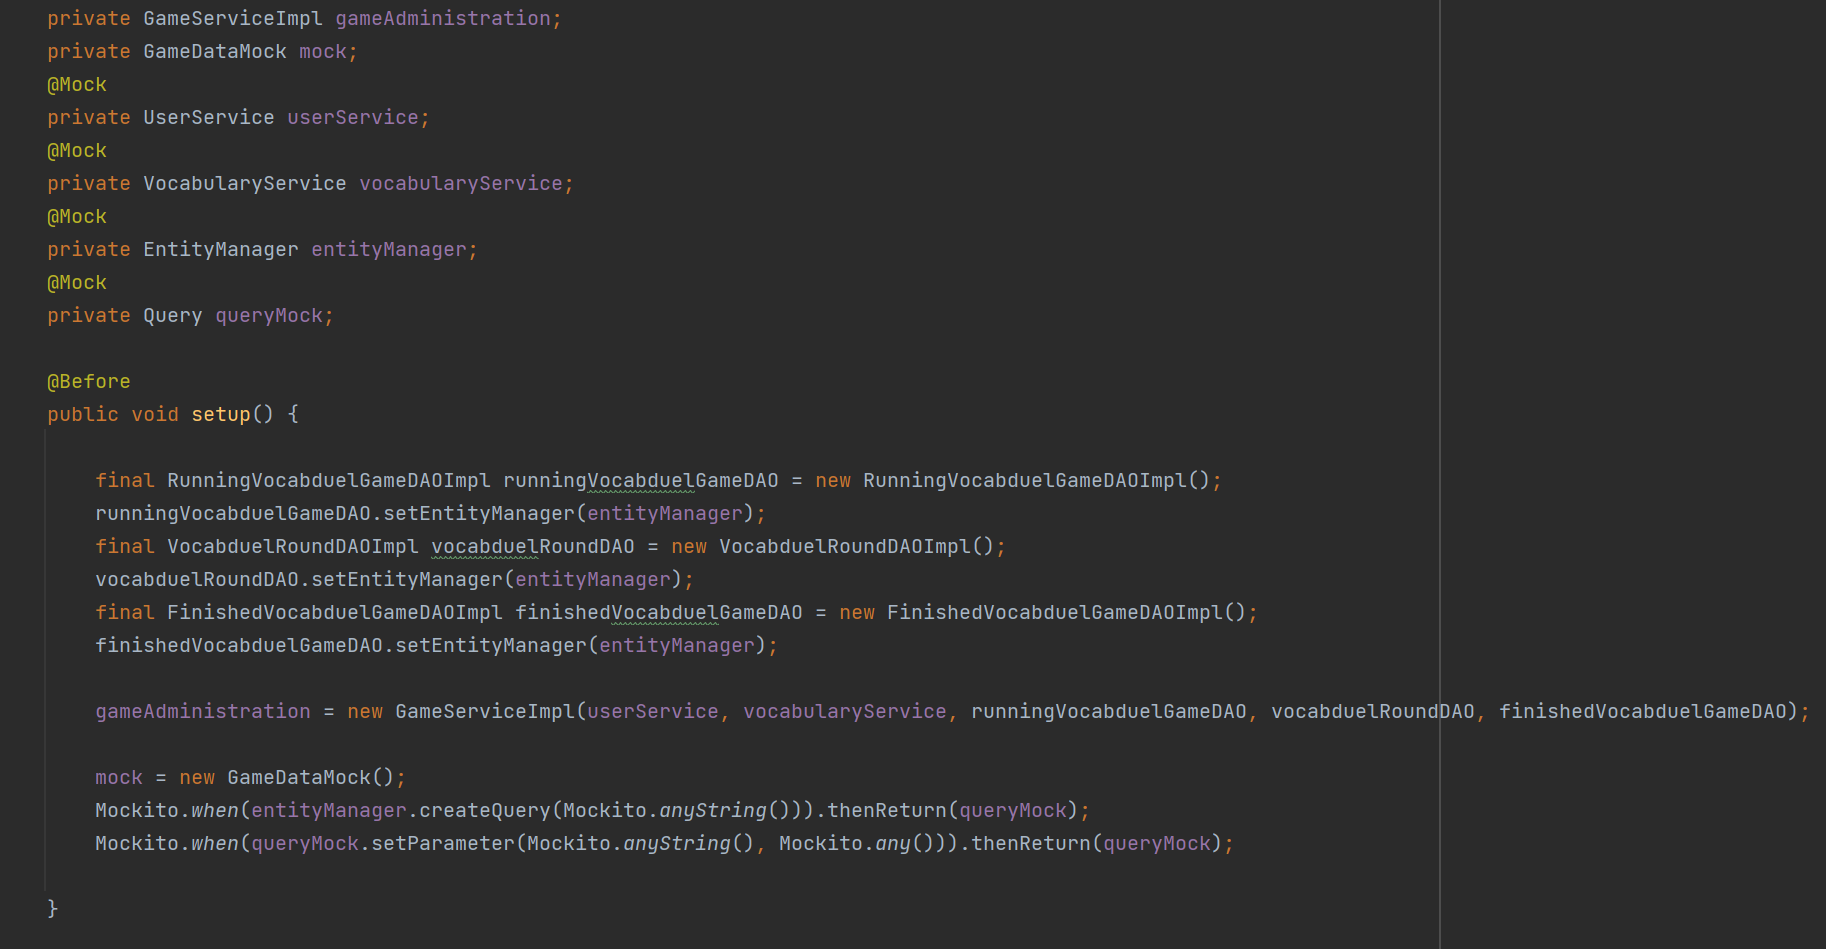
\includegraphics[width=0.8\textwidth]{mockito}
    \caption[]{Ausschnitt aus einer Testkonfiguration mit Mocks}
    \label{fig:mockito}
\end{figure}

Bei den InvalidPwdsTests und bei den ValidPwdsTests starten die Tests allerdings parametriesiert.

\begin{figure}[H]
    \centering
    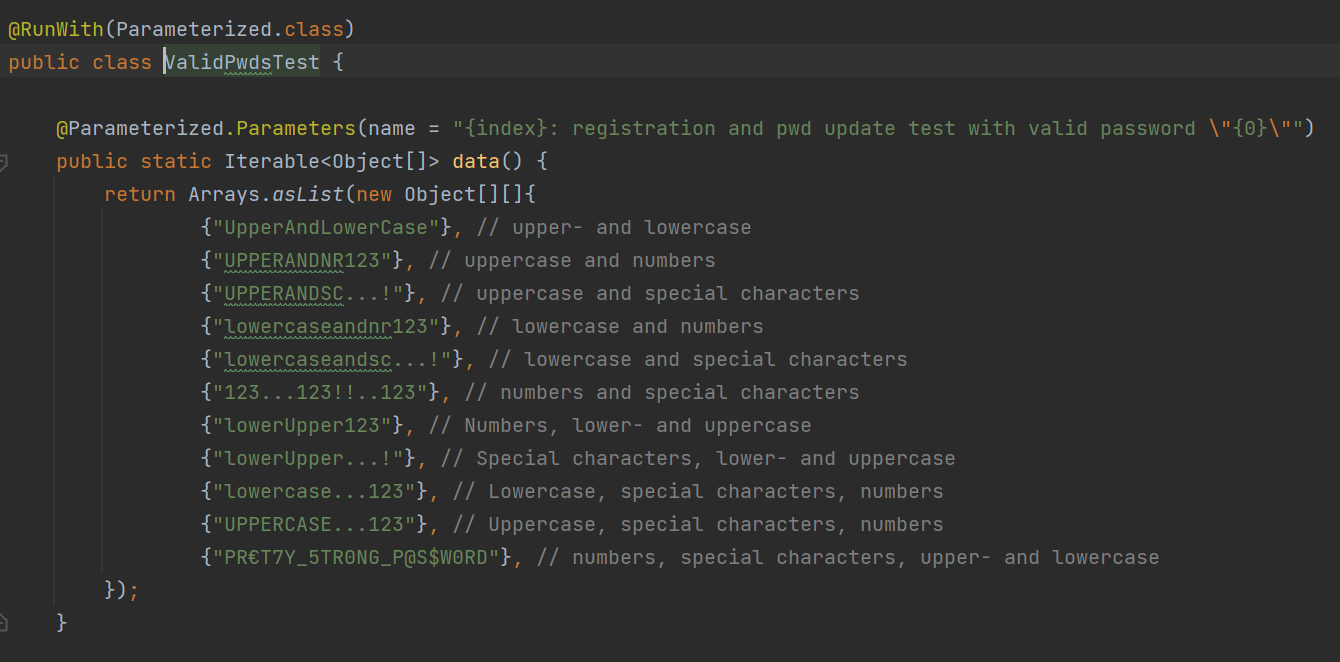
\includegraphics[width=0.8\textwidth]{param-test}
    \caption[]{Konfiguration einer parametrisierten Testklasse}
    \label{fig:param}
\end{figure}
    \section{Ablaufumgebung}\label{sec:ablaufumgebung}

\subsection{Voraussetzungen}\label{subsec:voraussetzungen}

\subsubsection{Maven}

Um das Projekt lokal aufzusetzen, wird \textit{Maven} in der Version \texttt{3.6} oder h\"oher ben\"otigt.
Ob bzw. in welcher Version \textit{Maven} bereits installiert ist, kann mithilfe des folgenden Befehls ermittelt werden:

\begin{lstlisting}[label={lst:mvnv}]
mvn -v
\end{lstlisting}




\subsubsection{MySQL}

Zus\"atzlich ist für die Datenverwaltung eine lokale \textit{MySQL}-Datenbank auf Port \texttt{3306} (default) erforderlich,
in der f\"ur den Nutzer \texttt{ROOT} das folgendes Passwort festzulegen ist: \texttt{Test\#-\#44}

Um die Datenbank aufzusetzen, gibt es wiederum zwei M\"oglichkeiten, die sich im Rahmen der Entwicklung als gleichermaßen geeignet erwiesen:

\begin{itemize}
    \item \textbf{Manuell:} Einrichtung mithilfe des MySQL Installers (\url{https://dev.mysql.com/downloads/}).
    \item \textbf{Docker:} Starten von MySQL als Docker Container.
    Folgender Befehl kann hierf\"ur genutzt werden:
\end{itemize}

\begin{lstlisting}[label={lst:dockerdb}]
docker run -p 3306:3306 -e MYSQL_ROOT_PASSWORD="Test#-#44" --name vdb -d mysql
\end{lstlisting}

Die Parameter \texttt{--name <...>} zur Namensgebung sowie \texttt{-d} zum Starten im detached-Modus sind empfohlen, aber optional.


\subsubsection{Tomcat Server}

Voraussetzung für die REST-API bzw. die Webanwendung ist zudem \textit{Tomcat Server} (getestet in Version \texttt{9.0.40}).

\subsection{Bauen der Anwendungen}\label{subsec:bauen-der-anwendungen}

Zum Intallieren aller Abhängigkeiten und zum Bauen der Module ist folgender Befehl auszuf\"uhren:

\begin{lstlisting}[label={lst:mvncleaninstall}]
mvn clean install
\end{lstlisting}

Mithilfe des Plugins \textit{frontend-maven-plugin}, genutzt im REST-Konfigurationsmodul, 
wird darüber hinaus in diesem Kontext direkt die Webanwendung gebaut.
Hierfür werden lokal \textit{Node/NPM} sowie \textit{Angular} installiert und
im Anschluss alle Abhängigkeiten der Frontendanwendung geladen und das Projekt gebaut. Ablage unter: 
\newline\texttt{./configuration.rest/src/main/webapp/app}

Somit sind \textit{Angular} bzw. \textit{Node/NPM} nur für die Entwicklung erforderlich, nicht aber zum Bauen aller Module. 
Alle für diese lokale Konfiguration geladenen Dateien werden in \texttt{./configuration.rest/node} gespeichert
(dieser Ordner wird von der Versionsverwaltung ignoriert).



\subsection{Starten der Anwendung}

\subsubsection{Konsolenoberfläche (veraltet)}

Um die als Konsolenanwendung implementierte Konfiguration zu starten, ist die \texttt{main}-Methode der 
Klasse \texttt{ConfigurationSpringImpl.java} des Moduls \texttt{configuration} als Java-Anwendung zu starten.
Es ist jedoch zu erwähnen, dass es sich hierbei um eine veraltete Implementierung handelt, der gegenüber die
im folgenden Kapitel beschriebene Konfiguration vorzuziehen ist.

\subsubsection{REST-API und Webanwendung}

Über das Modul \texttt{configuration.rest} lässt sich ein Server starten, der die REST-Schnittstelle sowie die Weboberfläche bereitstellt.
Hierfür ist die für dieses Modul generierte \texttt{war}-Datei in einer Tomcat-Konfiguration als zu deployendes Artefakt anzugeben.
Für die Nutzung in \textit{IntelliJ} liegt im Repository unter \texttt{./.run} eine direkt nutzbare Konfiguration für Tomcat \texttt{9.0.40} bereit.

Die von dem Modul bereitgestellte Webkonfiguration
\linebreak(\texttt{./configuration.rest/src/main/webapp/WEB-INF/web.xml}) sieht folgende Pfade vor:

\begin{itemize}
    \item \textbf{\texttt{<host>:<port>/api/...}}: REST-Schnittstelle
    \item \textbf{\texttt{<host>:<port>/app/...}}: Webanwendung
\end{itemize}

Ein großer Vorteil des Deployments auf demselben Server liegt darin, auf diesem Weg Cross-Origin-Zugriffe auszuschließen.
Für die lokale Entwicklung kann allerdings im Konstruktor der Klasse \texttt{ConfigurationRestEasyImpl} ein CORS-Filter konfiguriert werden.
Der Code hierfür ist im produktiven System jedoch aus Sicherheitsgründen auszukommentieren.

\begin{lstlisting}[label={lst:cors}]
CorsFilter corsFilter = new CorsFilter();
corsFilter.getAllowedOrigins().add("*"); // for dev mode only!
corsFilter.setAllowedMethods("OPTIONS, GET, POST, DELETE, PUT, PATCH");
SINGLETONS.add(corsFilter);
\end{lstlisting}

%---sources---
    \newpage
    \pagenumbering{Roman}

%---appendices---
% ?

\end{document}